\chapter{Experiments}\label{cap.experiments}


In this chapter we explain how we chose the elements of our algorithm and the results of it on the datasets.

\section{Validation experiments}\label{valdiation}



\subsection{Object detector}\label{valdiation:det}

For the choice of the detector we compare the detectors studied in the theoretical review on the \textit{MOT16} dataset. In the figure \ref{objectDetector2} we can observe the ROC curve of different detectors.



\begin{figure}[H]
\centering         
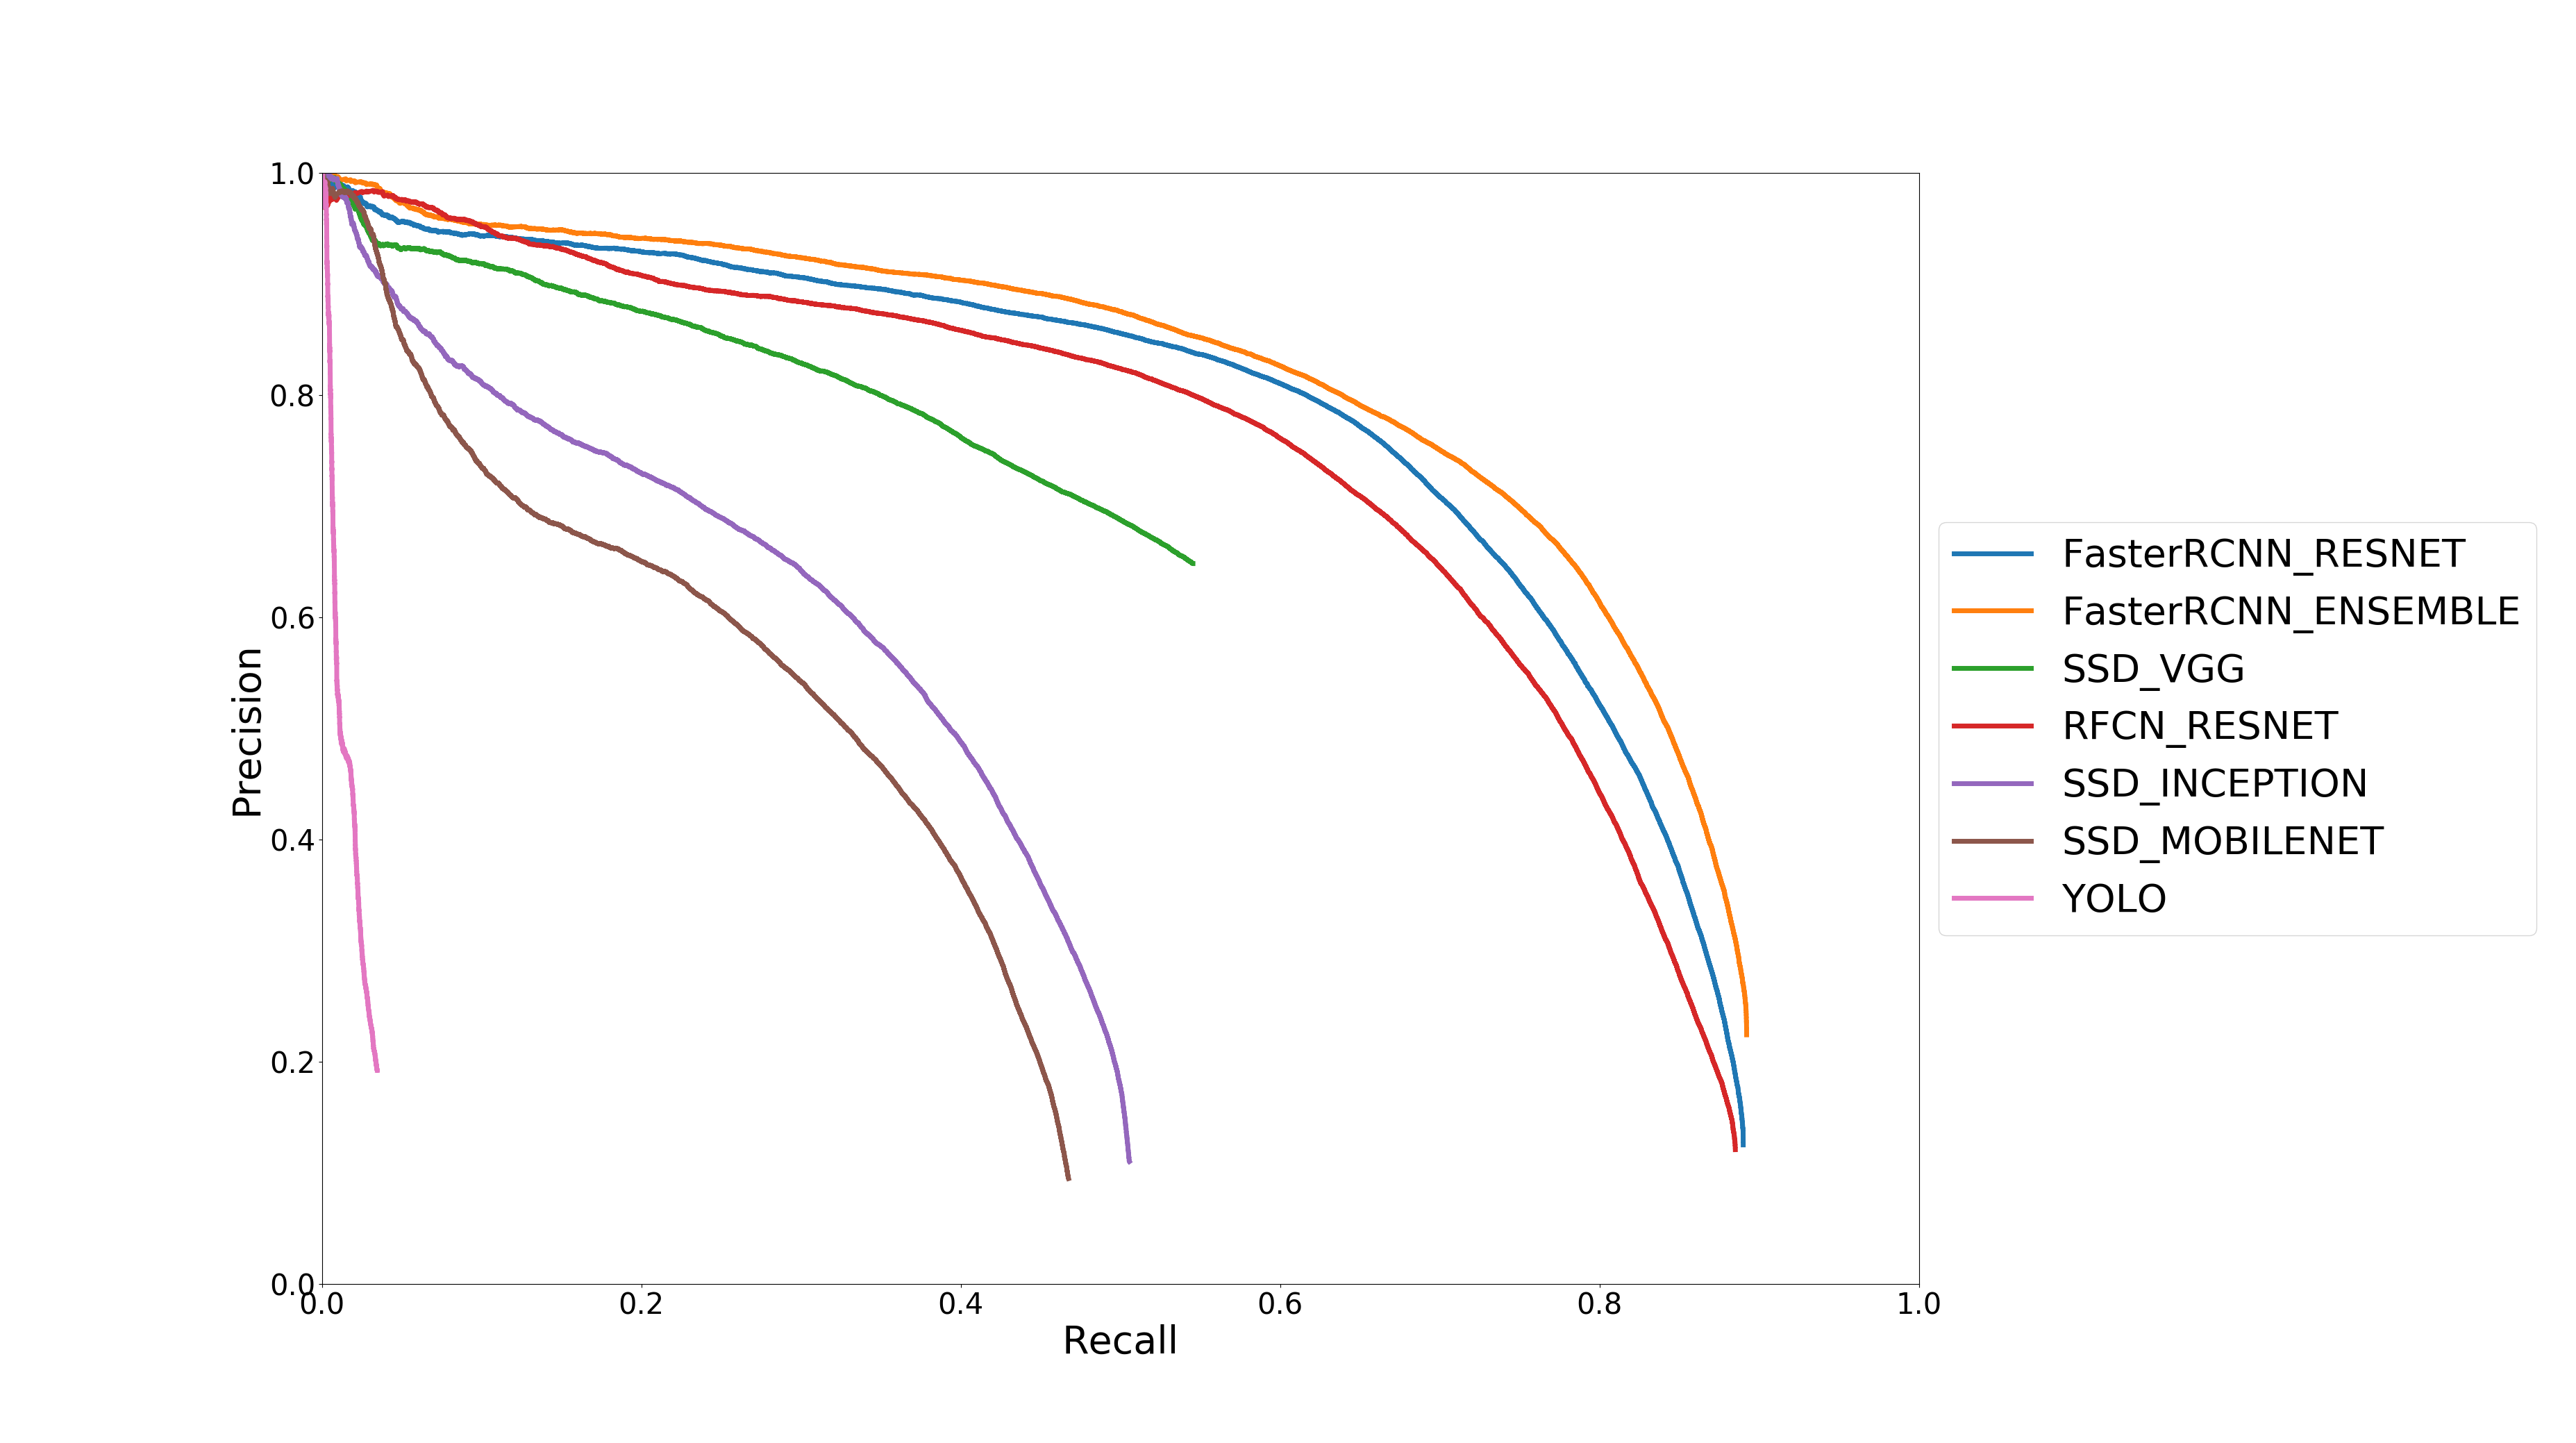
\includegraphics[width=0.9\linewidth]{evaluacionObject/dadas.png}
\caption{Barplot of the timming.} \label{timing1}
\end{figure}

\begin{figure}[H]
\centering         
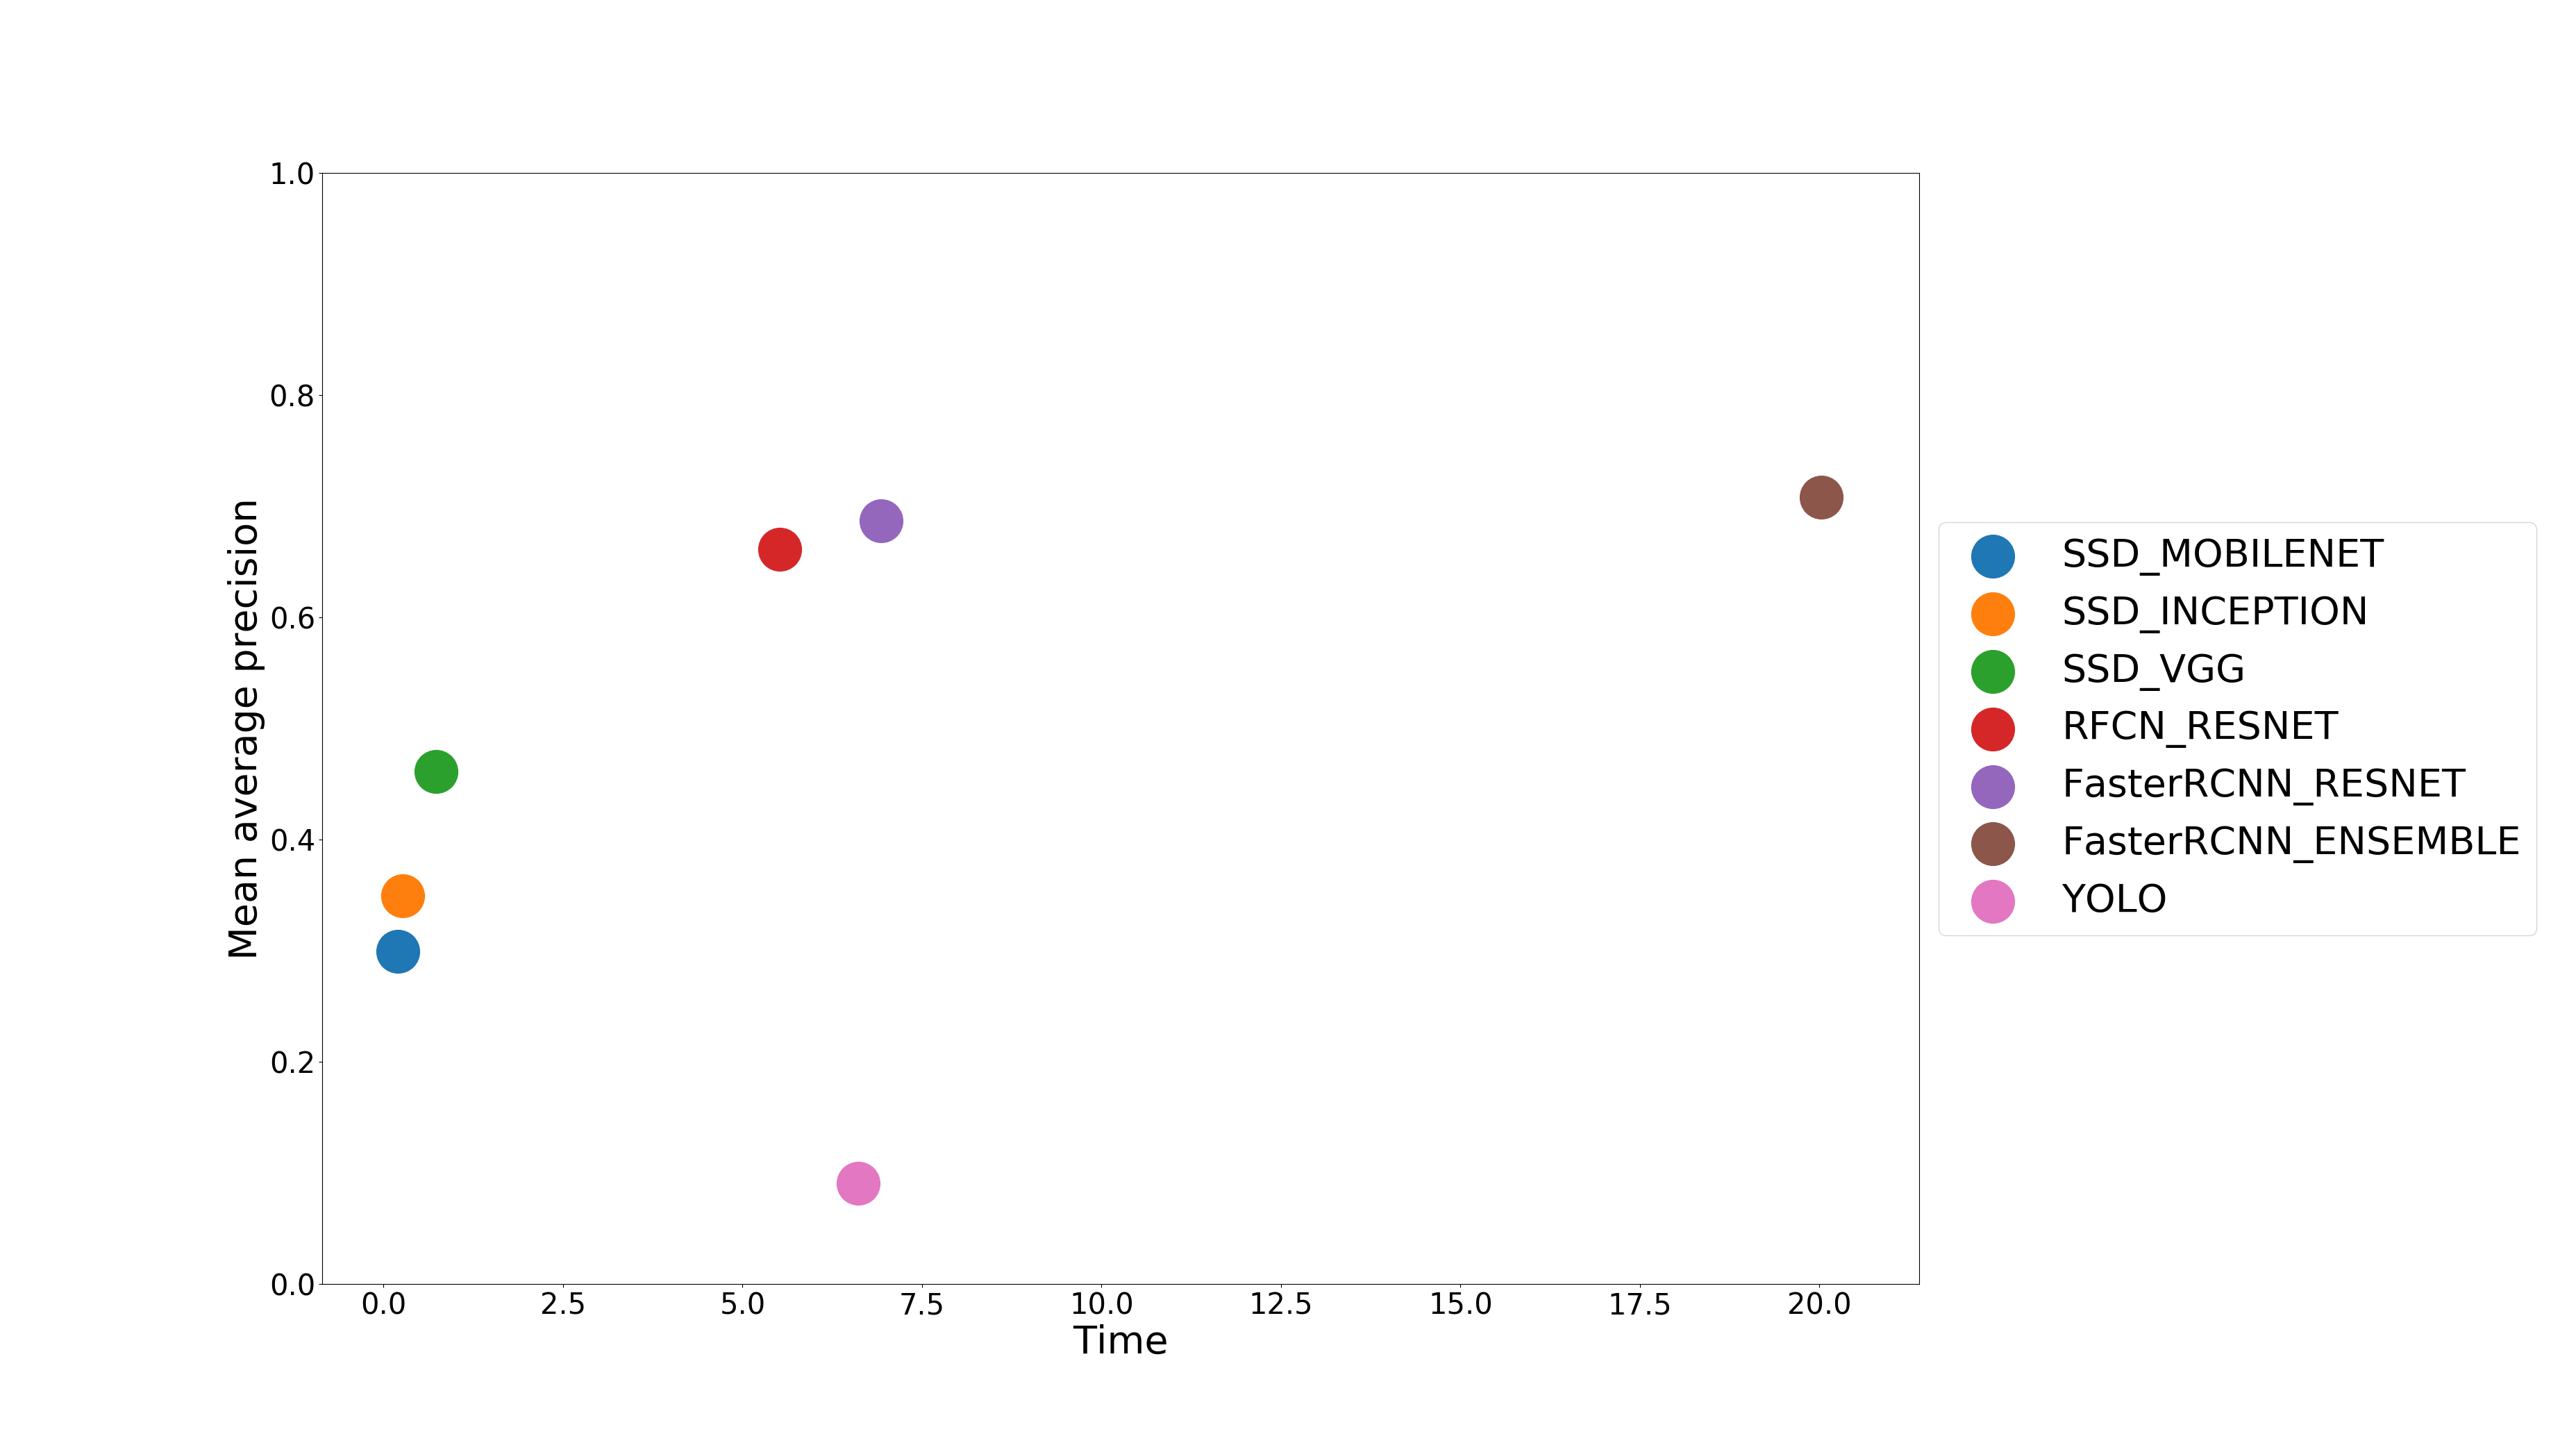
\includegraphics[width=0.9\linewidth]{evaluacionObject/meanAverage2.png}
\caption{Barplot of the timming.} \label{timing1}
\end{figure}



Finally, the conclusions of the characteristics are the following:

\begin{itemize}

\item \textbf{Faster-RCNN}, it scores $0.81$ average precision on the dataset, although we could not used due a software incompabilities, it requires a Nvidia GPU to be executed.

\item \textbf{R-FCN}, the code is not publicly available.

\item \textbf{DPM}, it scores $0.69$ average precision on the dataset, although we could not used due a software incompabilities, it requires a Nvidia GPU to be executed.

\item \textbf{YOLO}, it scores $0.09$ average precision on the dataset, it takes $6$ seconds per image \cite{yoloDark}. 

\item \textbf{PVANET}, the code is not publicly available.

\item \textbf{SSD}, it scores $0.73$ average precision on the dataset, it takes $0.9$ seconds per image. We used the tensorflow version of the detector \cite{ssdCode} instead of the original code \cite{ssdCode2}.


\end{itemize}

According to these results we chose the SSD detector, as object detector on this thesis.

\subsection{Tracking module}


The tracking module is inspired by the well-known tracking algorithm \textit{MedianFlow} by Zalal et al\cite{medianFlow} with his correspondent implementation in Python\cite{medianFlowPython}. Next we explain the tracking module in details.

According to \cite{visualTrackingSurvey}, our method belong to tracking using matching, considering that the algorithm performs a matching of the representation of the target model built from the previous frames. We do not build an additional extended model of the appearance and merge it with the matching, instead we will apply an object detector to correct the drift of the matching.


The tracking using matching is based on the optical flow, explained in \ref{TheoriecArch}, it computes the new position through gradient descent in several frames. We will assume that the motion is pure translational. As we can observe in the sequences of frames \ref{track1w} of the dataset, the pedestrians move in translation way in the image plane, so this assumption is achieved. 


\begin{figure}[H]
\centering         
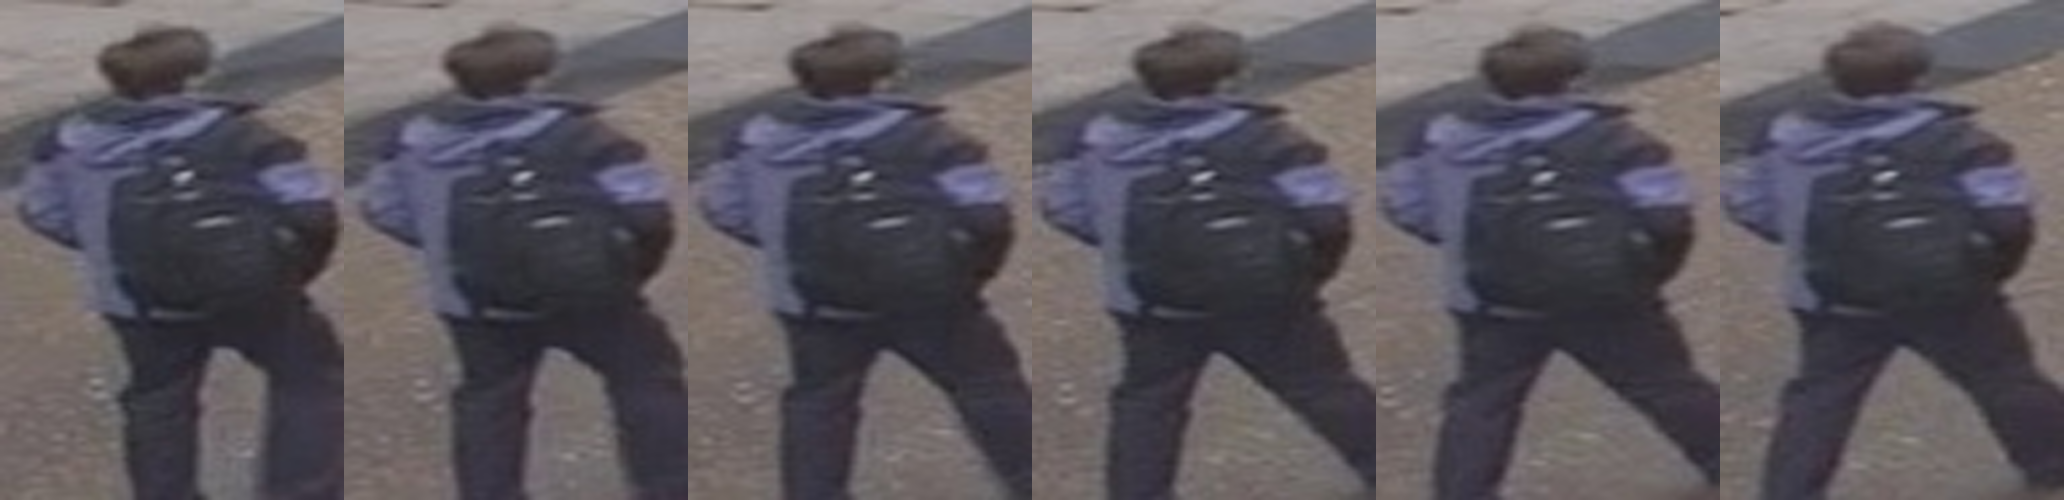
\includegraphics[width=0.9\linewidth]{changeCamera/tomeu.png}
\caption{Sequence of translational movement.} \label{track1w}
\end{figure}

In contrast to the previous figure, we can observe the next figure \ref{track2w} where the assumption of translation motion is not fulfilled ( this sequences does not belong to the used dataset, only showed to contrast the previous idea) and a translational assumption will failed.

\begin{figure}[H]
\centering         
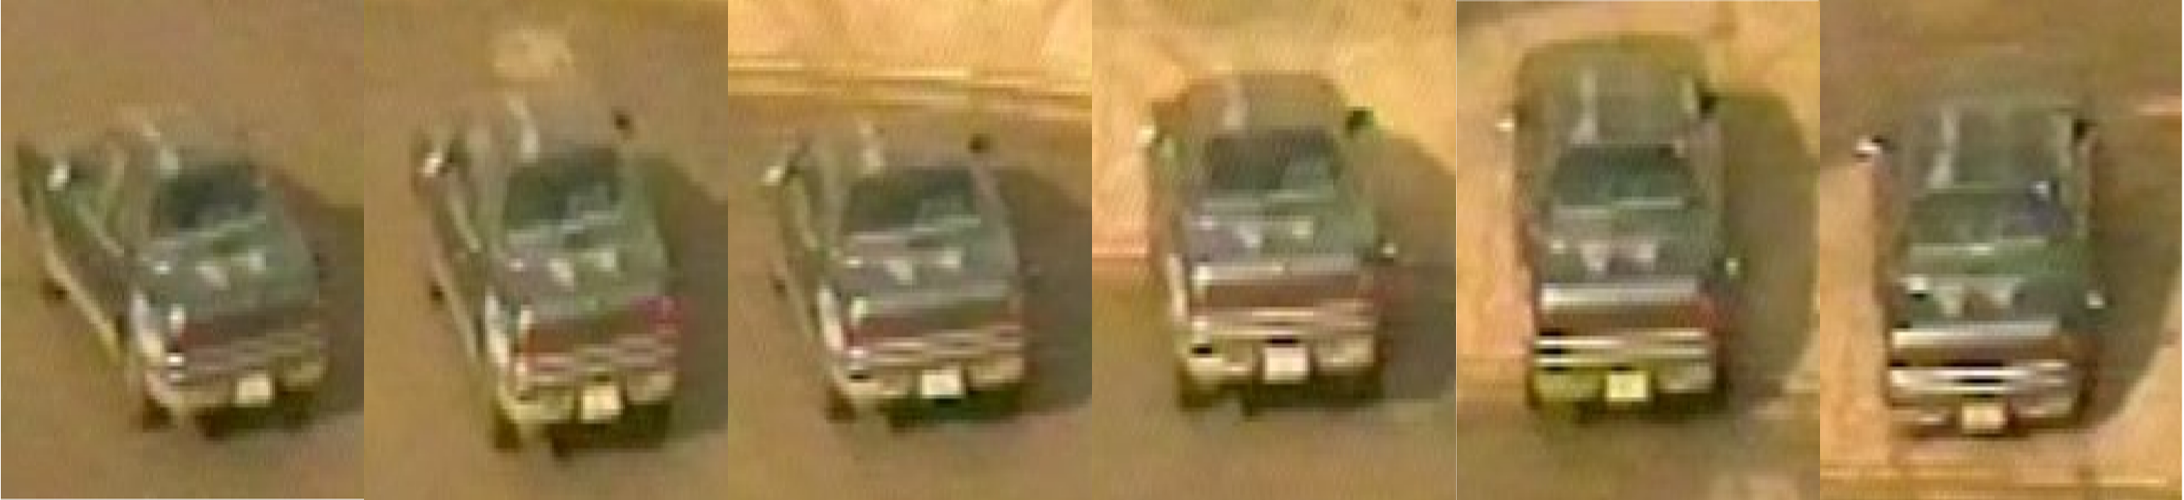
\includegraphics[width=0.9\linewidth]{changeCamera/out2.png}
\caption{Sequence of no translational movement.} \label{track2w}
\end{figure}





\subsubsection{Feature extraction}\label{exper:validation}

The strength of the further processing depends on the quality and quantity of this features, so in other to improve both, we apply some prepreprocessing to the image. We tried several preprocessings techniques like sharpening, image contrast, median filter, and equalization. In \ref{track1w}, we can observe the relation between number of points extracted and time comsuption of those techniques.




\begin{figure}[H]
\centering         
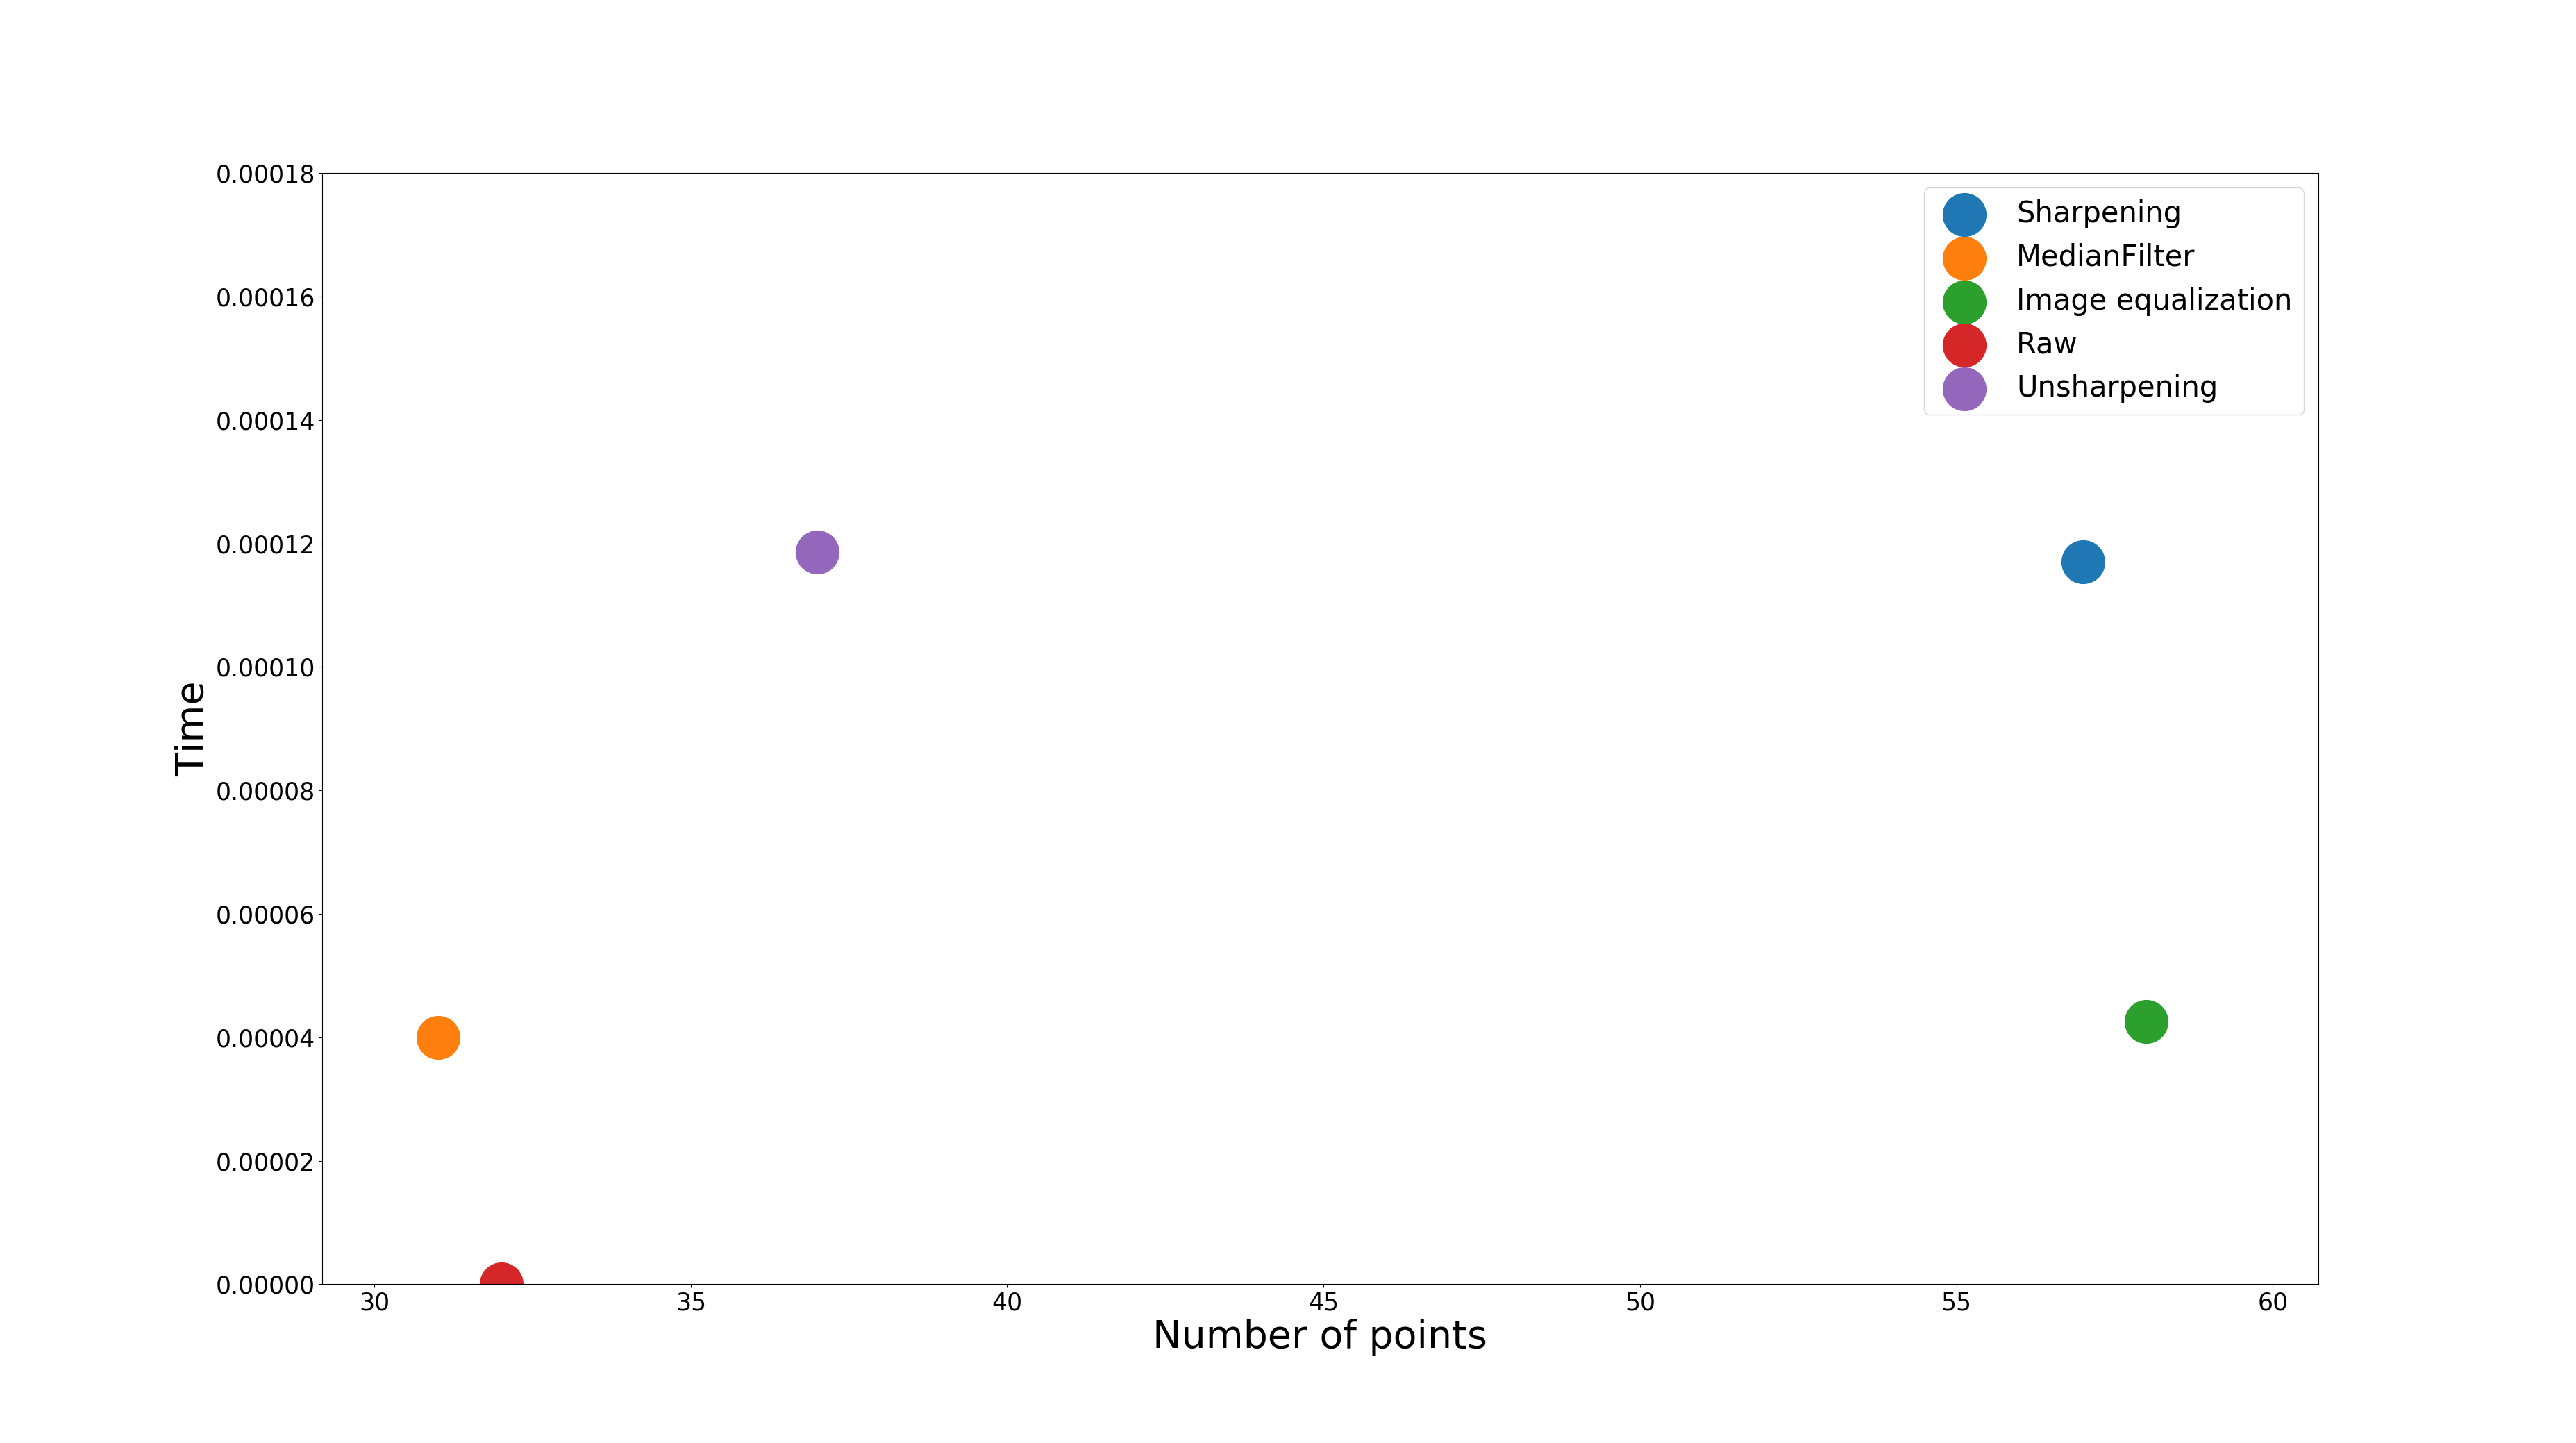
\includegraphics[width=0.9\linewidth]{tracker/preprocesing.png}
\caption{Barplot of the timming.} \label{timing1}
\end{figure}

We realized that the best preprocessing in terms of speed and number of points, is to equalize the image. The computation is really simple, it only consists in equalize an histogram and apply that transformation to the image. It increases over $ 55 \%$ the number points in comparision to not apply it to the raw image. In the figure \ref{prepoes} we can observe the different number of features in the raw and in the equalized image.

\begin{figure}[H]
		
\centering

\subfigure[Raw image.]{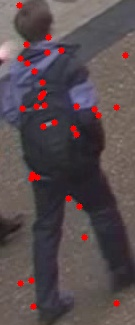
\includegraphics[width=3cm]{implementation/pointsSIN_EQU.jpg}}
\subfigure[Equalaized image.]{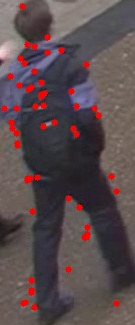
\includegraphics[width=3cm]{implementation/pointsEQU.jpg}}\\
\caption{Different preprocessings.}
\label{prepoes}
\end{figure}


\subsubsection{Matching module}


Forward backward

We used the Lucas-Kanade method to matching the points. Also, we implement the same method used in \cite{medianFlow}, the proposed method is based on so called forward-backward consistency assumption. That assumption consits in that correct tracking should be independent of the direction of time-flow. Algorithmically, the assumption is exploited as follows. First, a tracker produces a trajectory by tracking the point \textit{forward} in time. Second, the point location in the last frame initializes a validation trajectory. The validation trajectory is obtained by \textit{backward} tracking from the last frame to the first one. Third, the two trajectories are compared and if they differ signicantly, the forward trajectory is considered as incorrect. \ref{motion23} illustrates the method when tracking a point between two images. Point number $1$  is visible in both images and the tracker is able to localize it correctly. Tracking this point forward or backward results in identilcal trajectories. On the other hand, point number $2$ is not visible in the right image and the tracker localizes a different point. Tracking this point backward ends in a different location than the original one. We also implemented the forward method.



\begin{figure}[H]
		
\centering

\subfigure[Image forward-backward.]{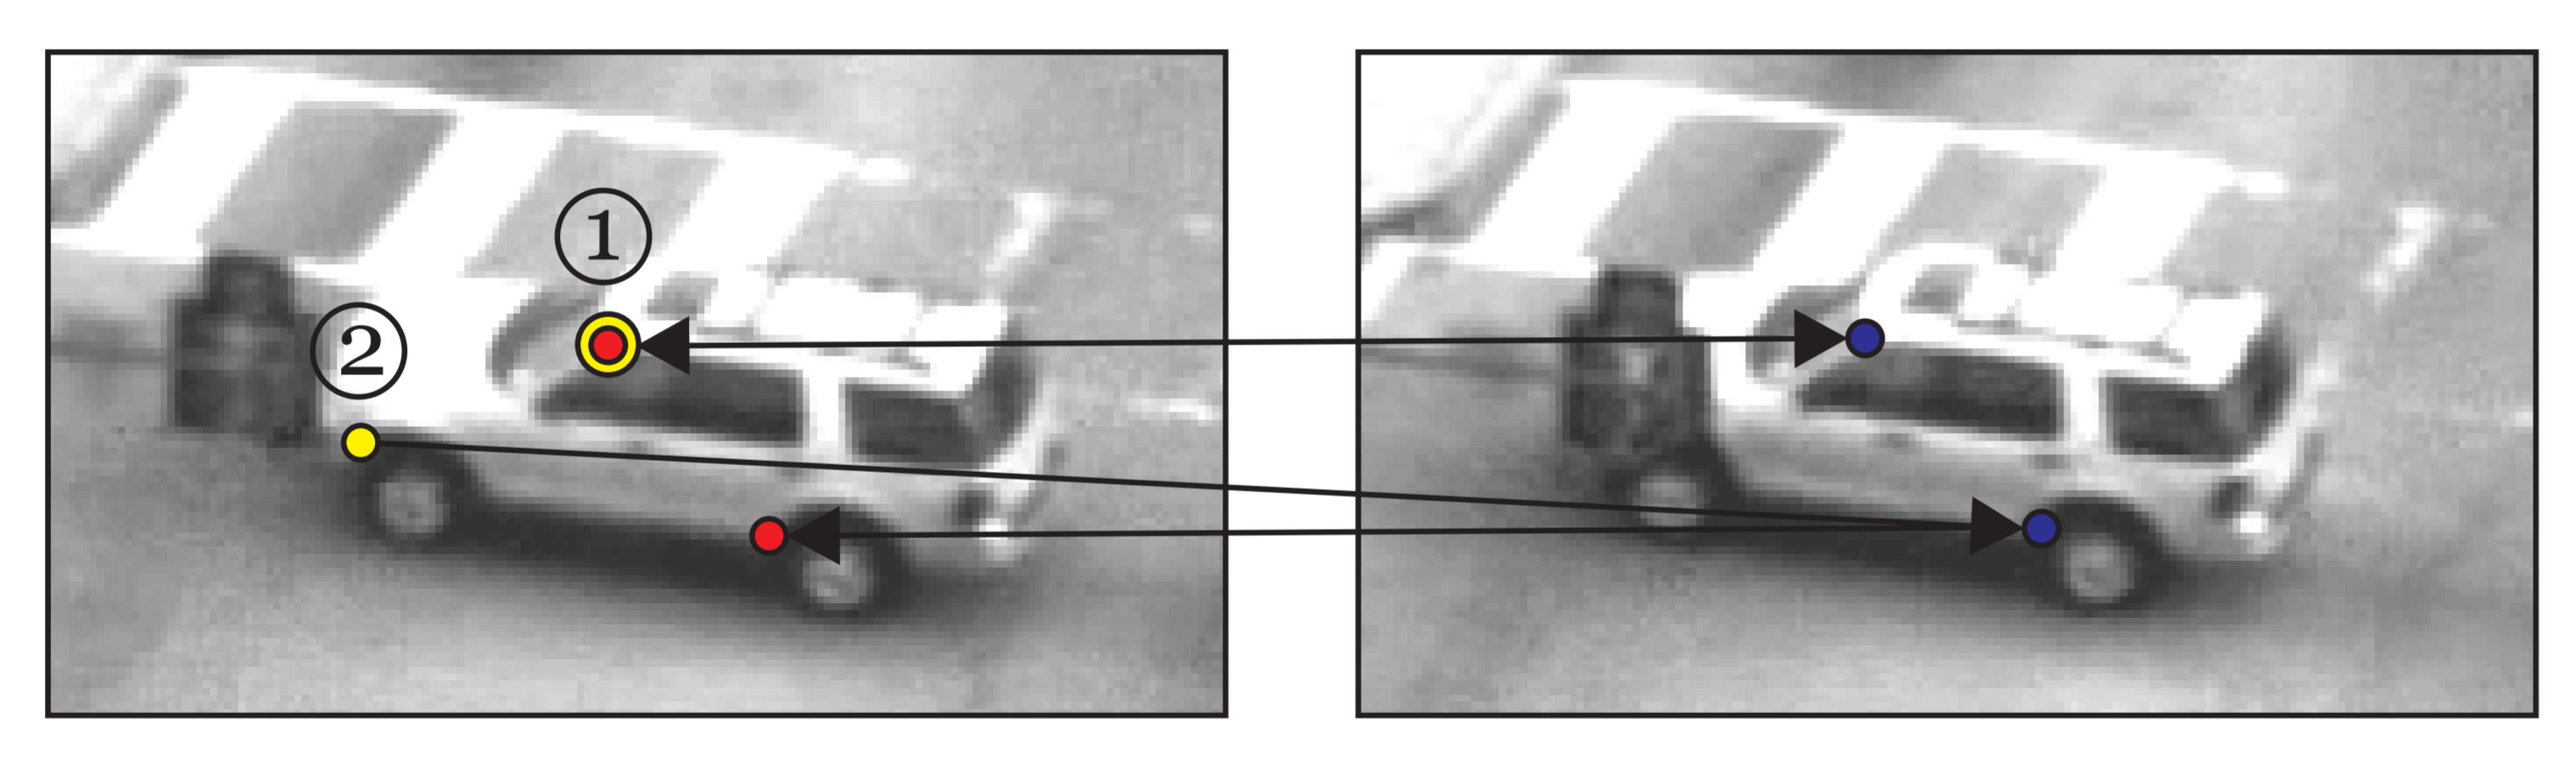
\includegraphics[width=7cm]{tracker/forwardBack.png}}
\subfigure[Scheme forward-backward.]{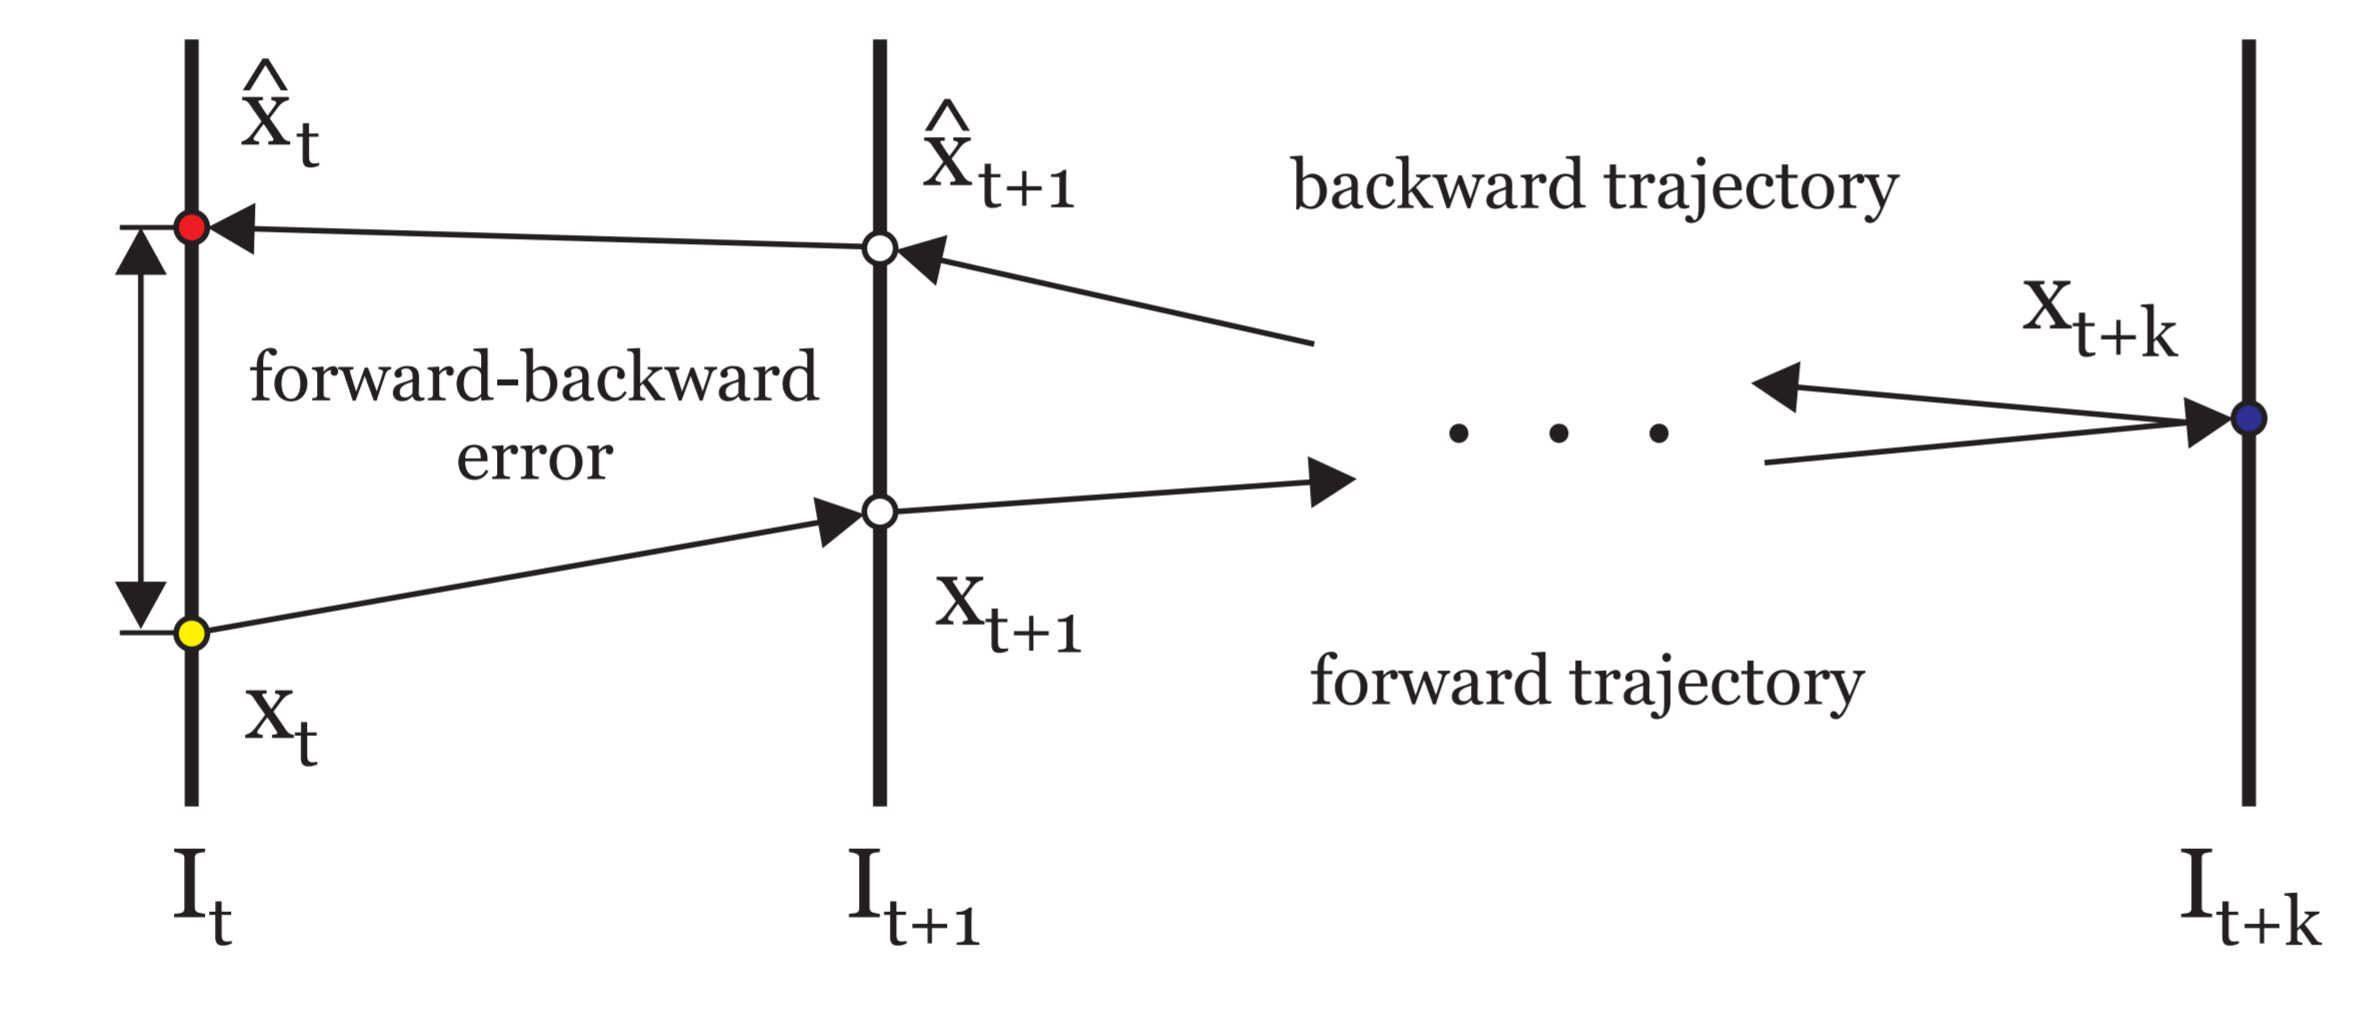
\includegraphics[width=7cm]{tracker/forwardBack2.png}}\\
\caption{Ilustration forward backward error.}
\label{motion23}
\end{figure}

\subsection{Siamese networks}\label{exper:entrenar}


To mantain the identity of the pedestrian we need a method to compare miss trackets with no associated detections. So, we decided to solve it with deep learning techniques, the scheme that we considered are the following:


\begin{itemize}


\item \textbf{Siamese network: Cost function}, this is based on the idea of deep learning as feature extractor and top layers as classifier. Two branches that share parameters process the images and classify it.

\item \textbf{Siamese network: In-network}, this is a mix of the previous models, where the information of the convolutional layers merges at some point before the classifier.

\item \textbf{Siamese network: Joint data input}, according to the literature this architecture gives the best results compared with the other topologies. The input of the network is aa concatenation of the two images and the network proces together.


\item \textbf{Feature extractor with cosine distance}, we used well-known architectures for image classification to extract features from the images and then compare those features with the cosine distance.

\item \textbf{Famous network fine-tuned}, we extract features for each image with a well-known architecture and merge it with a fully connected layer.

\end{itemize}

We can observe this architectures in the figure \ref{siameseData1}.

\begin{figure}[H]
		
\centering

\subfigure[Cost function.]{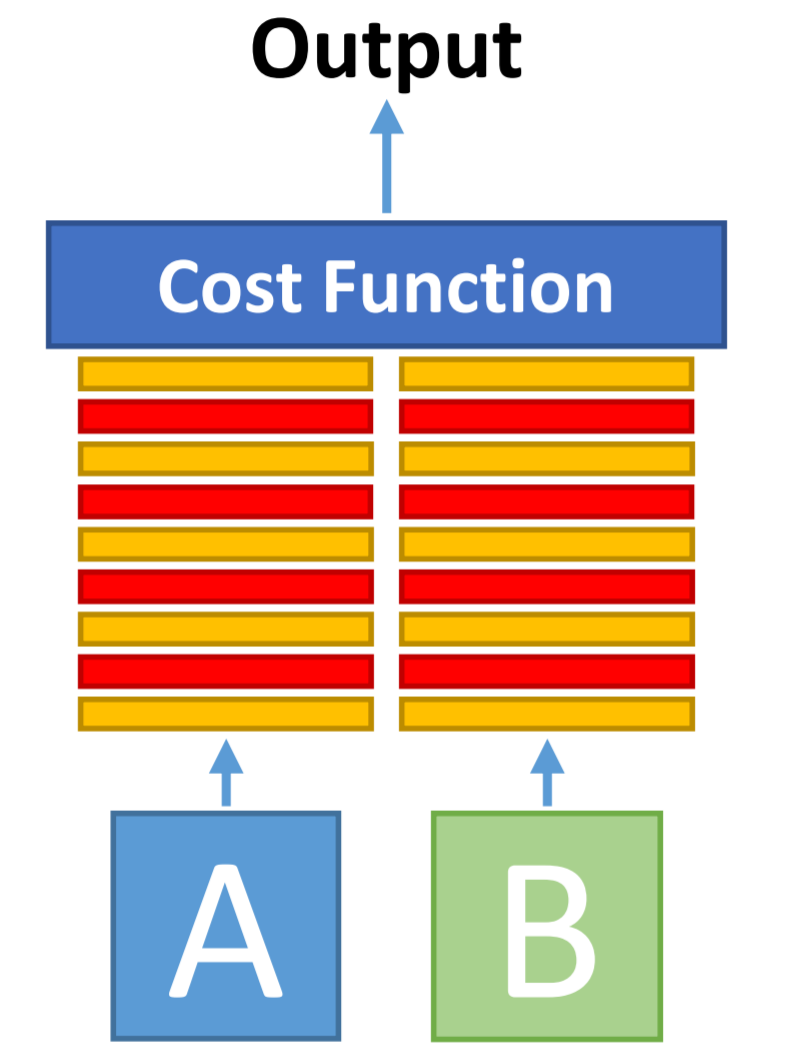
\includegraphics[width=2.7cm]{siamese/retall1.png}}
\subfigure[In-network.]{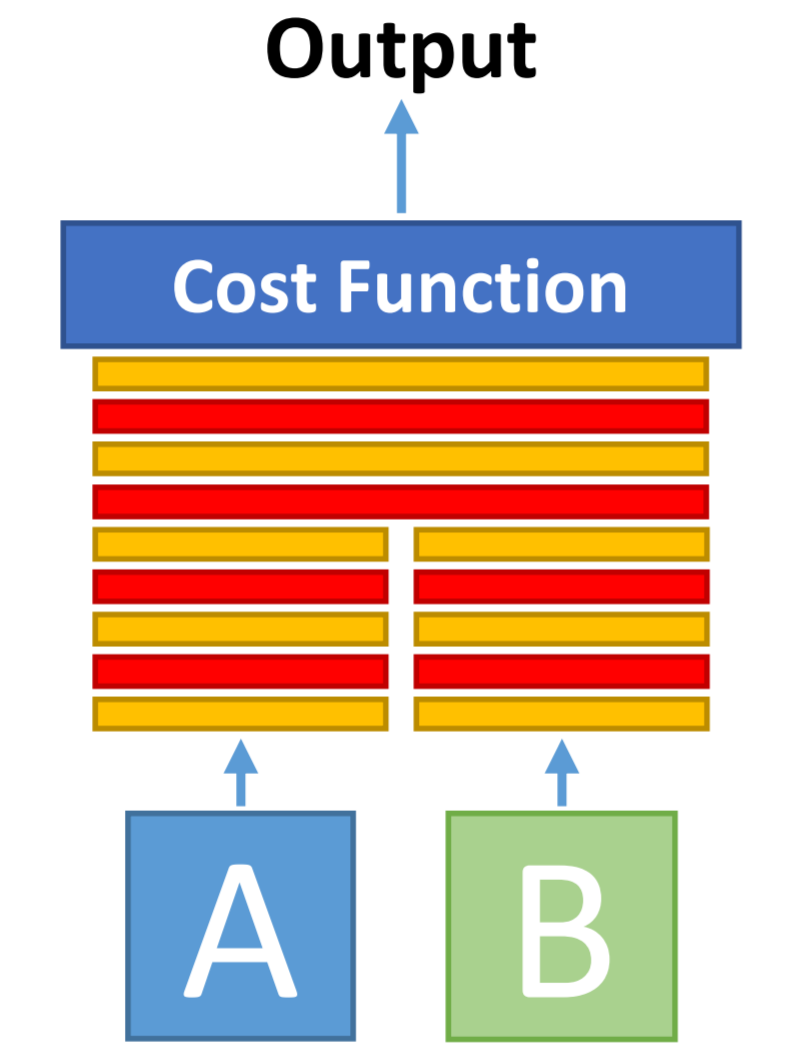
\includegraphics[width=2.7cm]{siamese/retall2.png}}
\subfigure[Joint data input.]{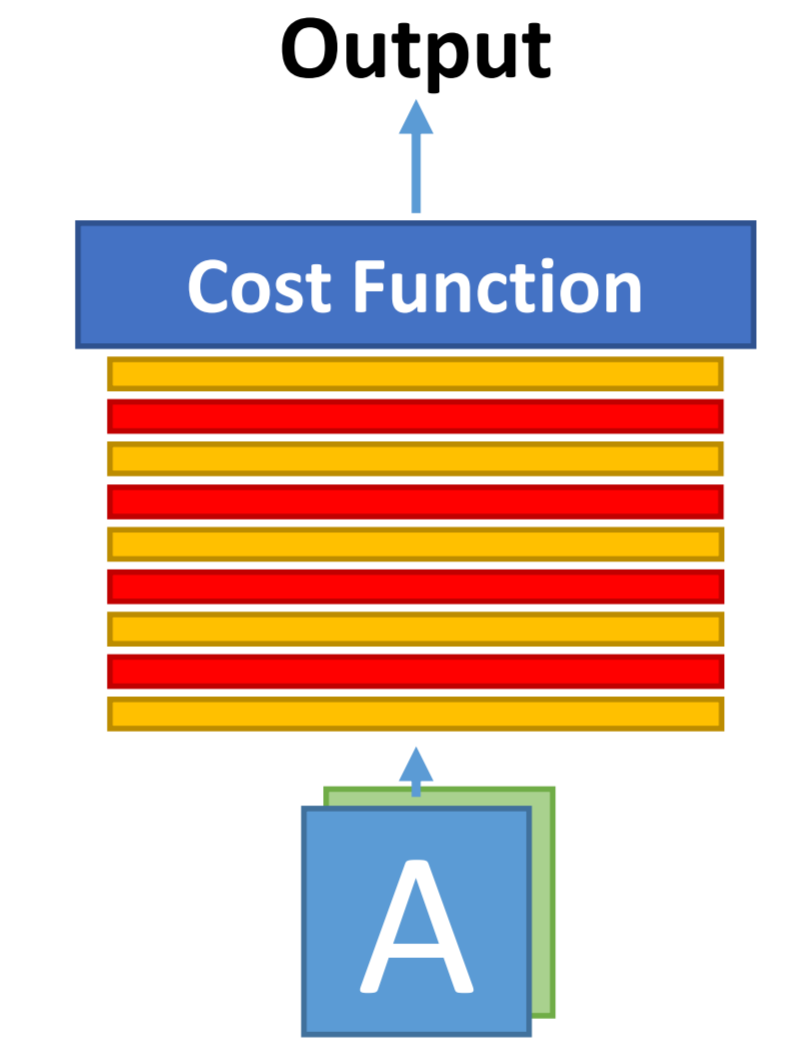
\includegraphics[width=2.7cm]{siamese/retall3.png}}
\subfigure[Features with cosine distance.]{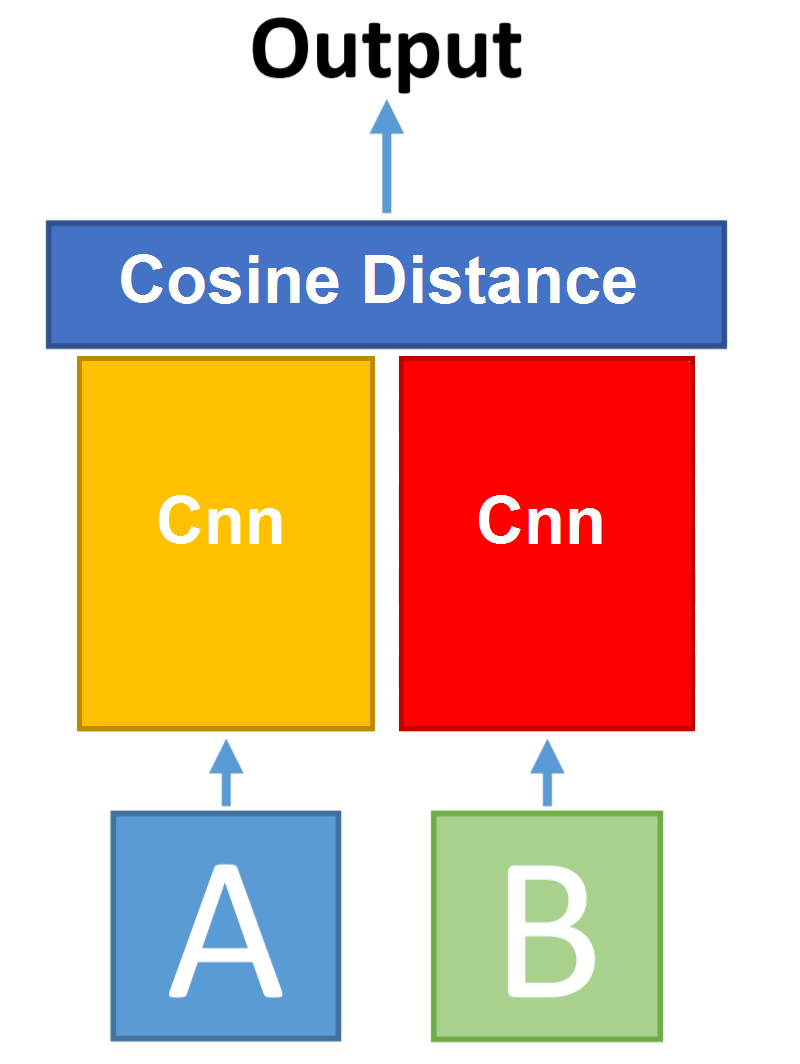
\includegraphics[width=2.7cm]{siamese/cosineDistance.png}}
\subfigure[Cnn fine-tuned.]{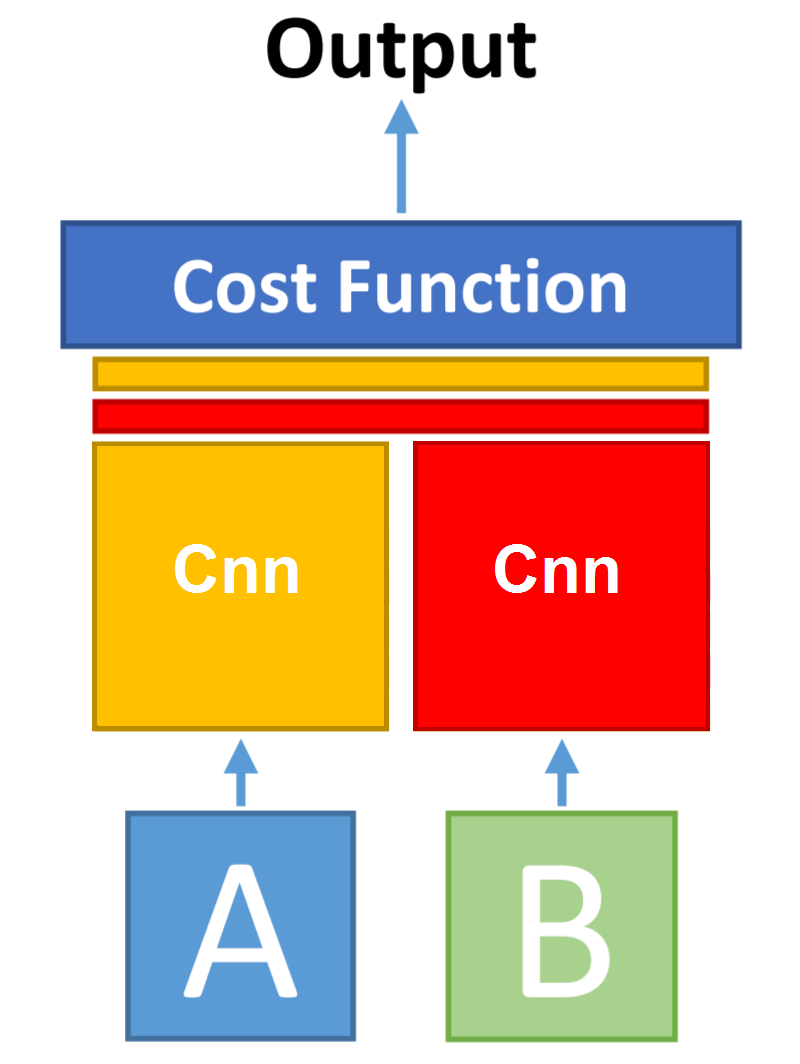
\includegraphics[width=2.7cm]{siamese/retall2cnnMAss.png}}\\


\caption{Siamese CNN topologies.}
\label{siameseData1}
\end{figure}


The main characteristics of the trained networks are the following:

\begin{itemize}

\item \textbf{Loss}, we used the binary cross entropy as a loss, we tried with the contrastive divergence but it did not converge.

\item \textbf{Optimizer}, As optimizer we used Adam, even though it has a mechanism to decrease the learning rate, we add a exponential decay, it speed up the convergence

\item \textbf{Activation}, we used ReLu. Currently, there other activations functions, but ReLu has been stablished as the reference.

\item \textbf{Inizialization}, To initialize the wrights we used He. inizialization, in adition we initialize the biases with the value of $0.1$, in this way we avoid the dead neurons in the firsts iterations.

\item \textbf{Batch normalization}, We tested batch normalization, but it adds to much computation time and we discarded it.

\item \textbf{Regularization}, we use Dropout in the fully connected layer to avoid overfitting.


\item \textbf{Final layers}, In the junction between the convolutional layers and the fully connected historically, a flatten mechansihm of the tensor has been used, but it increases dramatically the number of neurons in the fully connected layer, and it shows problems to converge. From the publication of InceptionV3, it appears with a global average pooling layer, it computes the spatial average of each layer of the tensor, reducing the number of parameters. Also we used the spatial pyramid pooling layers, it consists in a multiresolution max pooling. We can observe those differences in ref{siameseData2}.

\begin{figure}[H]
		
\centering

\subfigure[Flatten.]{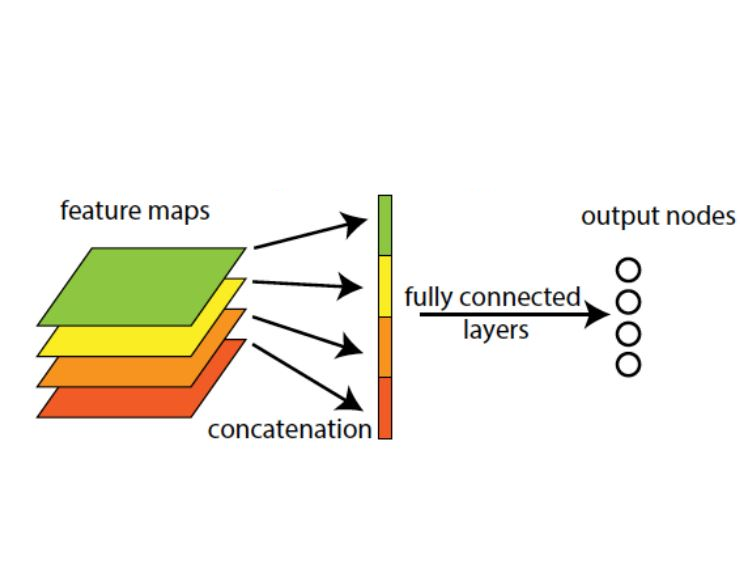
\includegraphics[width=4.5cm]{siameseDev/flatten2.png}}
\subfigure[Global average pooling.]{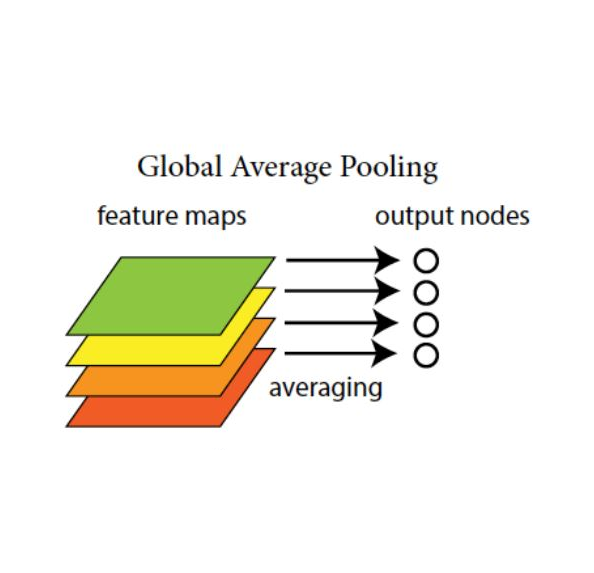
\includegraphics[width=4cm]{siameseDev/globalPooling.png}}
\subfigure[Spatial pyramid pooling.]{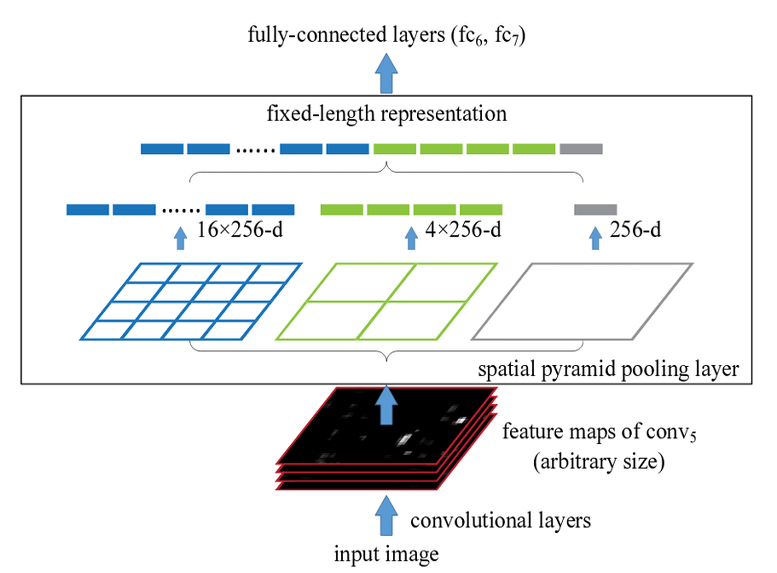
\includegraphics[width=4cm]{siameseDev/spp2.png}}\\



\caption{Final layers.}
\label{siameseData2}
\end{figure}


\item \textbf{Output}, We did not use softmax as ouput, we only used one neuron with sigmoid activation, in this way the output is constrainet between $0$ and $1$.



\end{itemize}


We developed our models in a VGG way, stacking  several convolutional layers and finishing it with a fully connected layers. We started with a few convolutional layers and added more till we reach an overfitting condition, this conditional will manifest when adding more layers the score on the test set decline. We started with $3$ and we end up with $7$ convolutional layer as best performance.

For the dataset, it does not exist a prominent dataset in the field, so we decided to use the MOT16 as dataset to adapt the domain. In order to do so, we extract the detections with their identities, and then for each identity we selected all possible random pairs and for the negative set we selected several random identites. The negative dataset is much bigger than the positive dataset, so we limited it to have a balanced dataset. The problem with the MOT16 dataset, is that the ground truth was built with the detections of a classifier and there is not a human intervention, resulting in a messy ground truth. We inspected the dataset and around the $70 \%$ of the dataset was wrong, there are a lot of oclussion in detection resulting in erronous pairs, pairs that are not matching with the same identity.

Then, we decided to discard the MOT16 dataset an use the TownCenter dataset \cite{townCenter} from the University of Oxford, which has got a manual ground truth. We have got $29824$ positive and negative pairs, then a dataset of $59648$ image pairs. We split the dataset between training and validation set, $80 \%$ and $20 \%$ respectively. For testing we selected a set of identities of the MOT16 dataset. To regularize and enlarge our dataset we applied some data augmentation techniques to our dataset like we observe in figure \ref{msii1}. For each pair we added one transformation, so we double our dataset. We tried to apply all the transformation for each images but the dataset was too noisy and the network did not converge.






\begin{figure}[H]
		
\centering

\subfigure[Original image.]{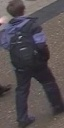
\includegraphics[width=2cm]{dataAugmentation/resizedImage.jpg}}
\subfigure[Random image brightness.]{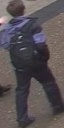
\includegraphics[width=2cm]{dataAugmentation/imageBrightnes.jpg}}
\subfigure[Random crop.]{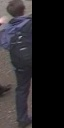
\includegraphics[width=2cm]{dataAugmentation/imageRandomCrop.jpg}}
\subfigure[Vertical flip.]{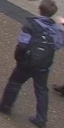
\includegraphics[width=2cm]{dataAugmentation/imageVerticalFlip.jpg}}
\subfigure[Gaussian blur.]{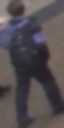
\includegraphics[width=2cm]{dataAugmentation/imageGaussianBlur.jpg}}
\subfigure[Random shadow.]{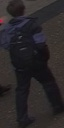
\includegraphics[width=2cm]{dataAugmentation/imageRandomShadow.jpg}}


\subfigure[Zoom in.]{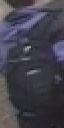
\includegraphics[width=2cm]{dataAugmentation/imageZoomIn.jpg}}
\subfigure[Rotation and translation.]{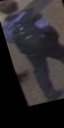
\includegraphics[width=2cm]{dataAugmentation/imageTransormed.jpg}}
\subfigure[Zoom out.]{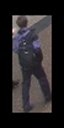
\includegraphics[width=2cm]{dataAugmentation/imageZoomOut.jpg}}
\subfigure[Gaussian noise.]{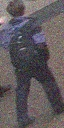
\includegraphics[width=2cm]{dataAugmentation/imageNoiseGaussian.jpg}}
\subfigure[Opposite vignetting.]{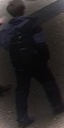
\includegraphics[width=2cm]{dataAugmentation/imageBLURcenter.jpg}}
\caption{Data augmentation.}
\label{msii1}
\end{figure}

We trained all the models and obtained a graphs like the figure \ref{lossesSiam}, we observe that the network converge, it decreases the loss and increases the accuracy, also we observe that tests plots are a little bit noisy, but we considered that the  regularization techniques are enough. We notice that the joint data input outperforms the other siamese configurations, so we increased the number of layers of that architecture, \textit{conv I}, refers to it, with $I$ the number of layers.

\begin{figure}[H]
		
\centering

\subfigure[Losses.]{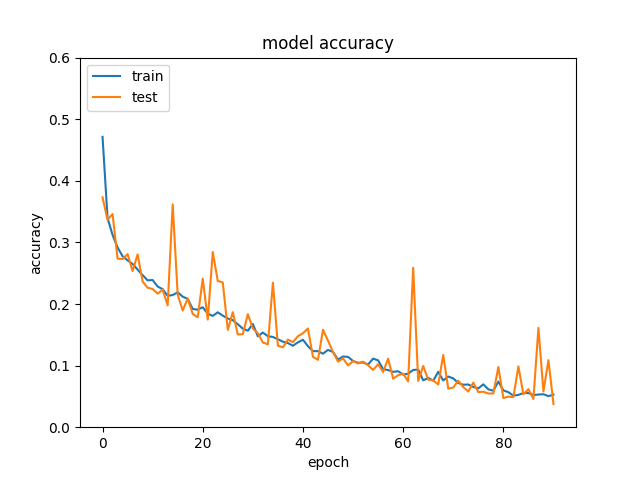
\includegraphics[width=7.5cm]{siameseDev/loss.png}}
\subfigure[Accuracy.]{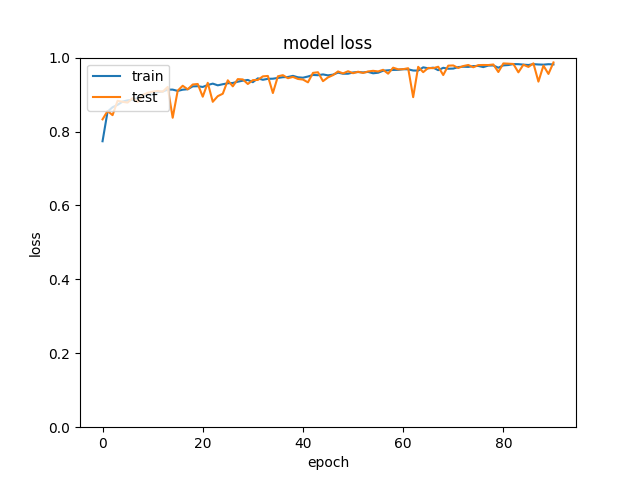
\includegraphics[width=7.5cm]{siameseDev/accuracy.png}}\\

\caption{Results training.}
\label{lossesSiam}
\end{figure}



Finally, we can observe the comparision using the CMC measure in the figure \ref{lossesSiam2}, we notice that the siamese network with joint data input with less layers than bigger models like Inception performs better, this remarks the idea of training jointly the feature extractor and the classifier and the need of task specific networks. Also, the siamese network with the configuration joint data input, outperforms the other siamese networks. Among the siamese joint data input, the performance increases till the $7$ convoltional layer architecture, then the $8$ convolutional layers drops.

\begin{figure}[hptb]
\centering         
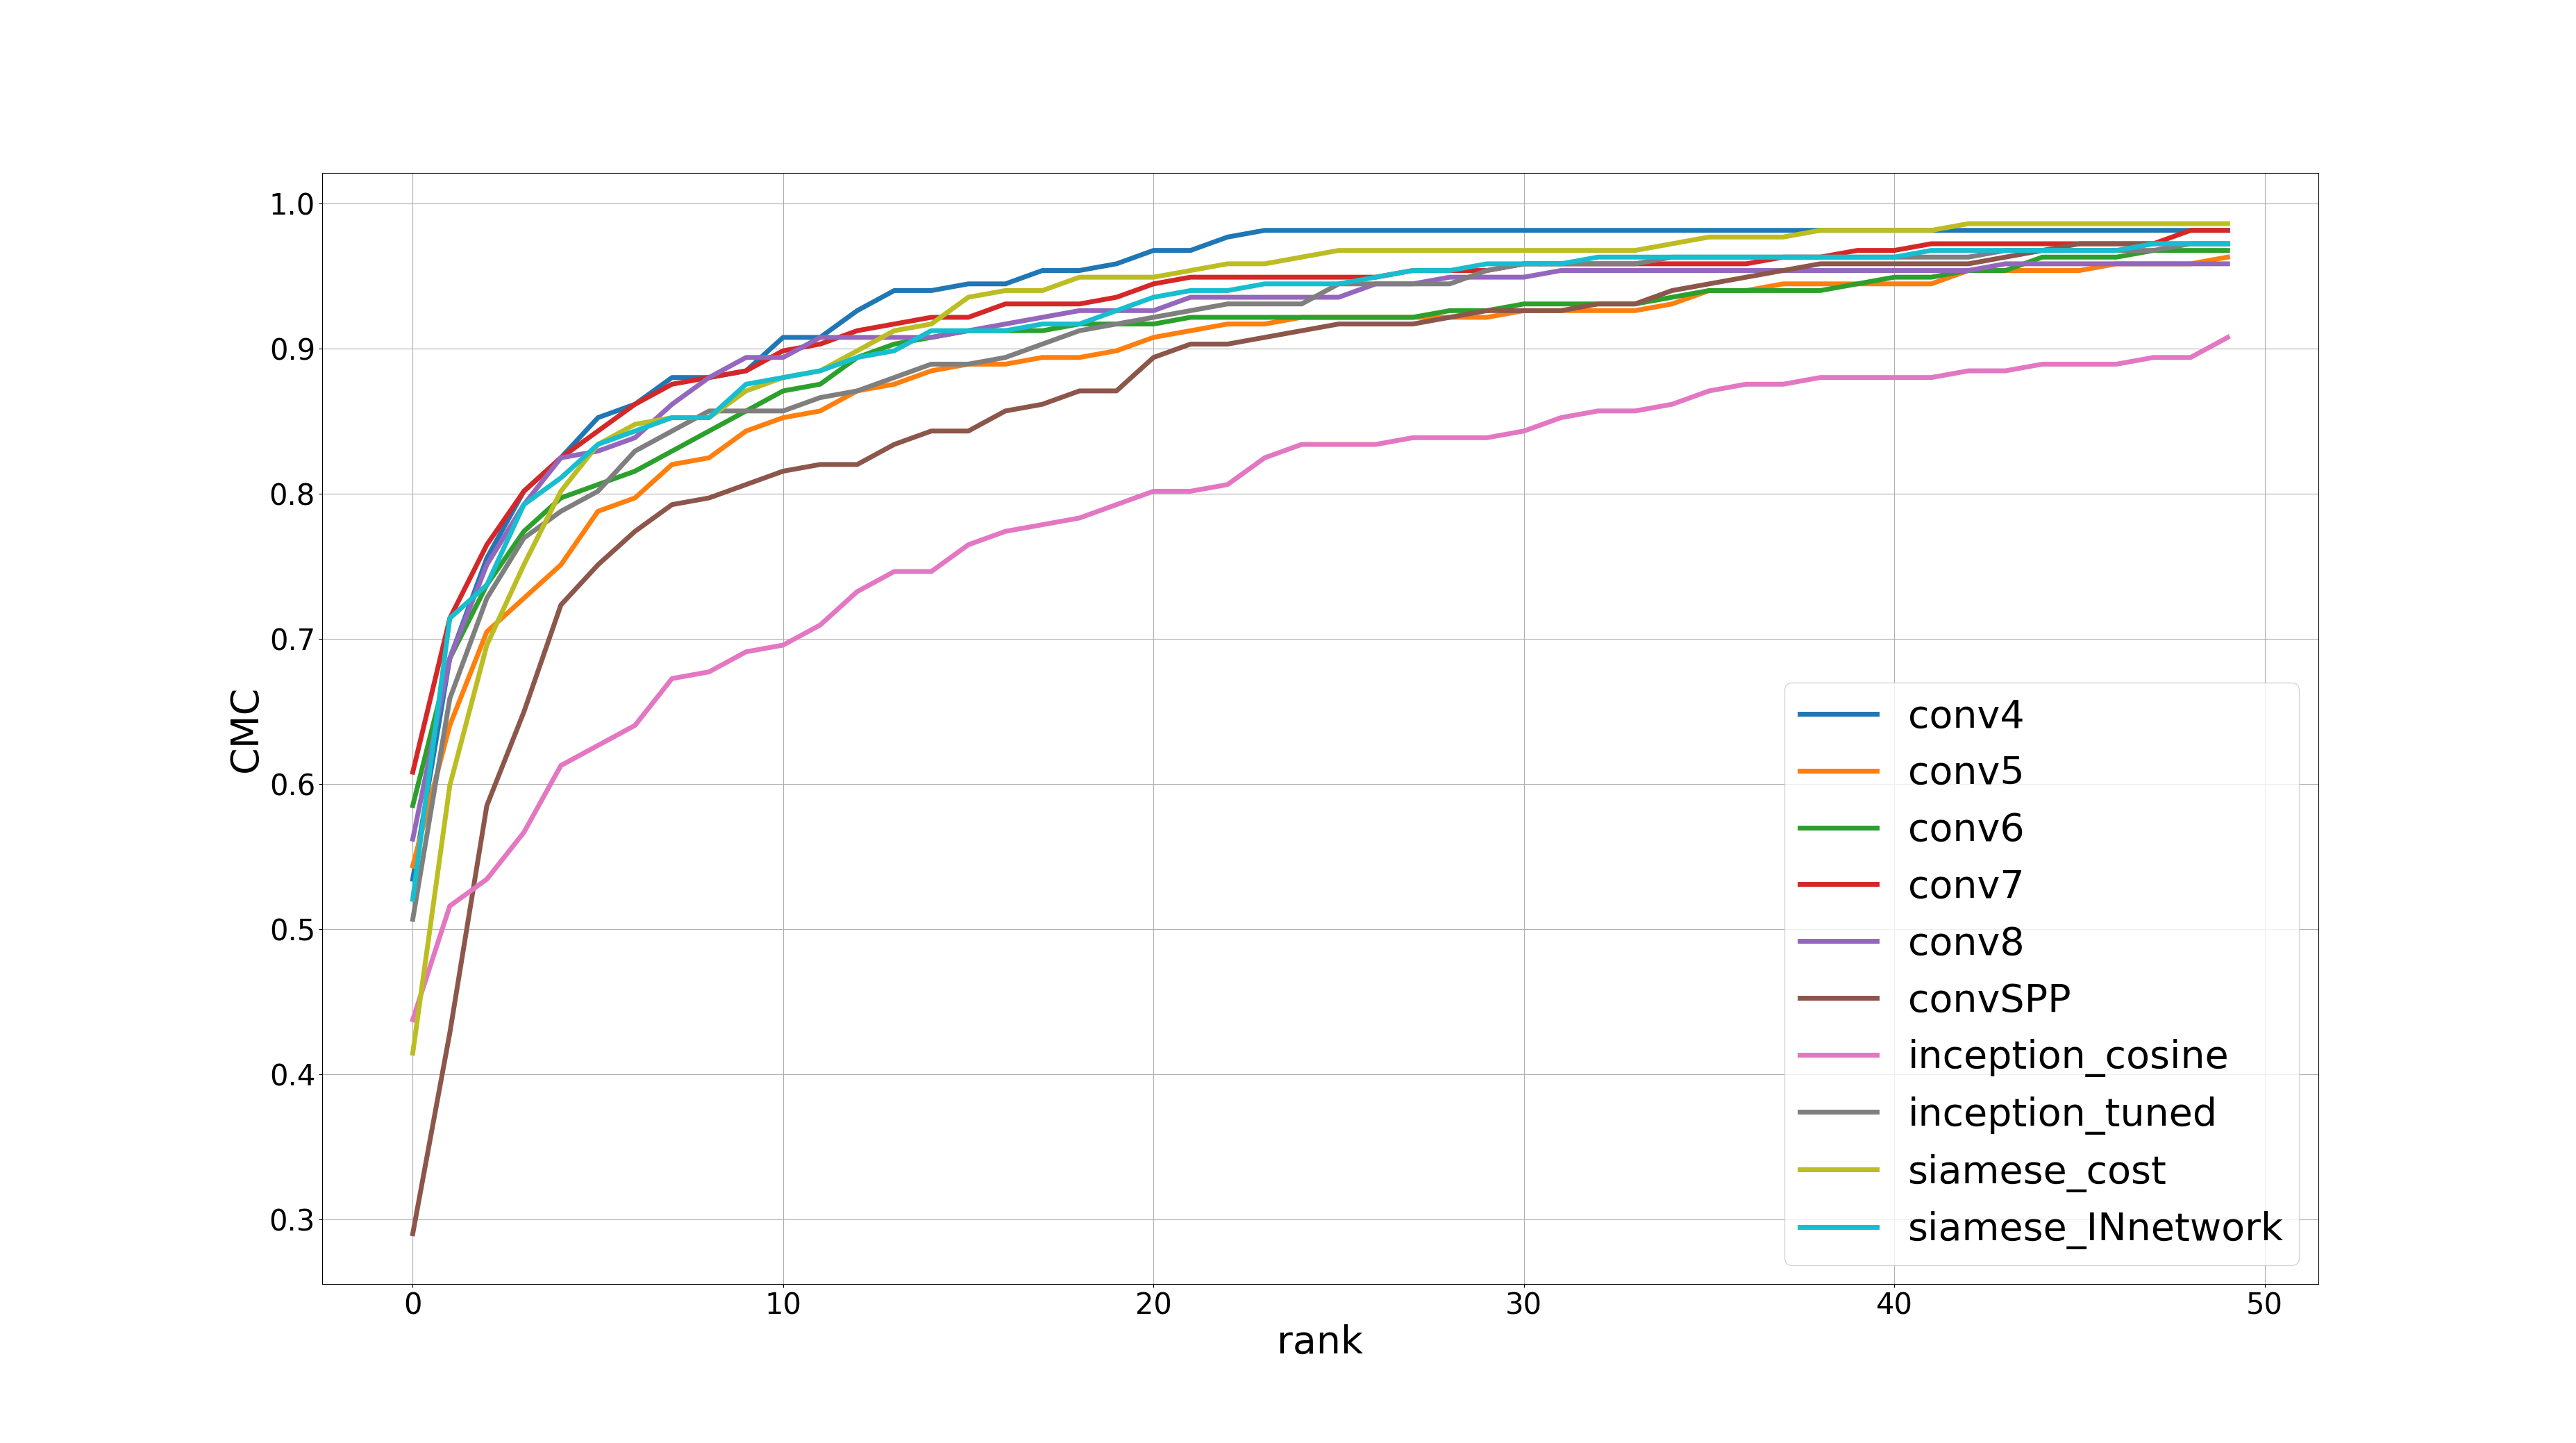
\includegraphics[width=12cm]{siameseDev/cmcNetwors.png}
\caption{CMC plot.} \label{lossesSiam2}
\end{figure}

Also in the next plot, we observe the performance against the time consumption the siamese network with the joint data input with $7$ convolutional layers gets the best balance between performance and execution time. 

\begin{figure}[hptb]
\centering         
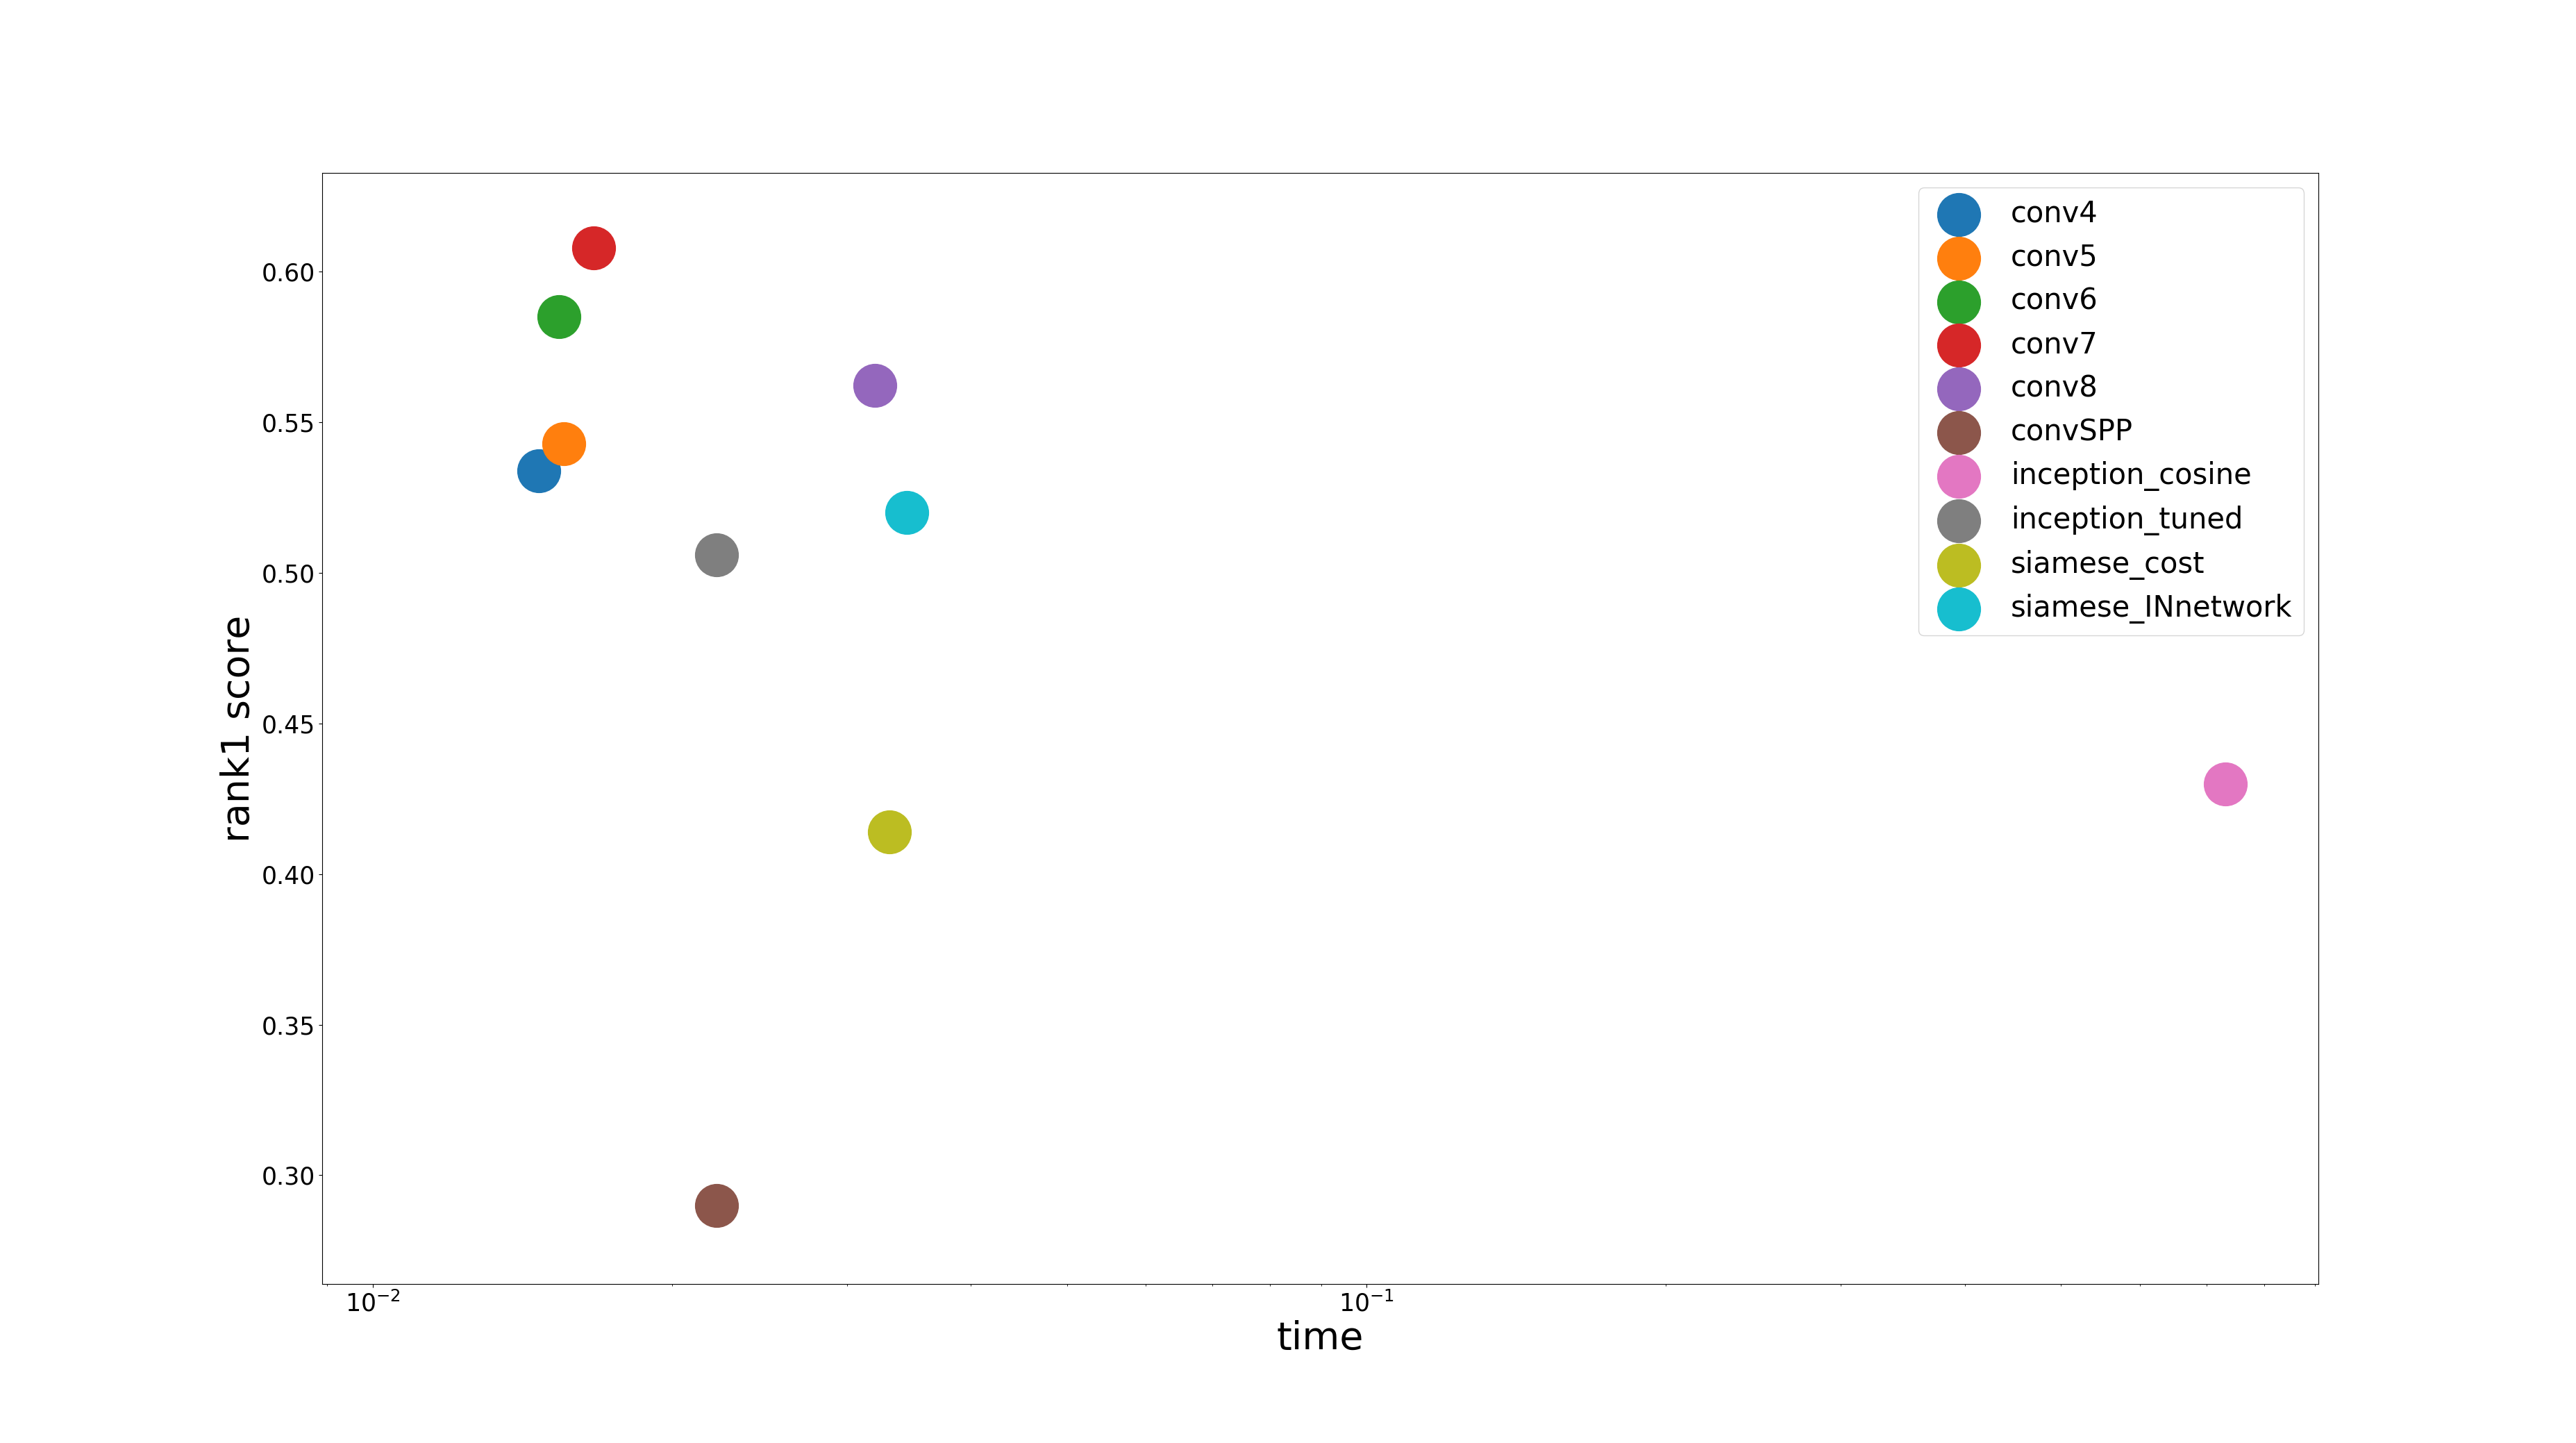
\includegraphics[width=12cm]{siameseDev/results.png}
\caption{Performance-timing comparision.} \label{lossesSiam3}
\end{figure}




\section{Algorithm evaluation}



In this section, we will analyse the performance and the timings of our solution.

\subsection{Performance}

Using the code provided by the MOT16 challenge organization, we evaluate our solution, we tested the version without re-identification module,\textit{v1}, the version with optical flow forward-bacward \textit{v2}, and the version with re-identification module and without forward-backward method, also we compare with the state of the art, an anonymous submission to the MOT16's website. The resulsts are showed in table \ref{tableResults}.


%\begin{table}[H]
%\centering
%
%\resizebox{\textwidth}{!}{\begin{tabular}{llll|llll|llll|llll}
%            & \textbf{Rcll} & \textbf{Prcn} & \textbf{FAR} & \textbf{GT} & \textbf{MT} & \textbf{PT} & \textbf{ML} & \textbf{FP} & \textbf{FN} & \textbf{IDs} & \textbf{FM} & \textbf{MOTA} & \textbf{MOTP} & \textbf{MOTAL} & \textbf{FPS} \\
%\textit{v1} & 24.4          & 49.5          & 5.17         & 517         & 12          & 180         & 325         & 27502       & 83462       & 827          & 1053        & 9.8          & 69.3          & 6,5        & 17,2   \\
%\textit{v2} & 19.6          & 61.8          & 2.52         & 517         & 3           & 127         & 387         & 13373       & 88754       & 618          & 936         & 10.8          & 70.3          & 7.5  & 15,85                                        
%\end{tabular}}
%\caption{Results algorithm global.}
%\label{tableResults}
%\end{table}


\begin{table}[H]
\centering

\resizebox{\textwidth}{!}{\begin{tabular}{llll|llll|llll|llll}
              & \textbf{Rcll} & \textbf{Prcn} & \textbf{FAR} & \textbf{GT} & \textbf{MT} & \textbf{PT} & \textbf{ML} & \textbf{FP} & \textbf{FN} & \textbf{IDs} & \textbf{FM} & \textbf{MOTA} & \textbf{MOTP} & \textbf{MOTAL} & \textbf{FPS} \\
\textit{v1}   & 21.4          & 49.5          & 5.17         & 517         & 12          & 180         & 325         & 13339       & 78998       & 827          & 1053        & 9.8           & 69.1          & 6.5            & 18.2         \\
\textit{v2}   & 21.3          & 50.4          & 5.12         & 517         & 11          & 181         & 325         & 11212       & 75738       & 827          & 1056        & 9.7           & 67.3          & 6.1            & 9.0          \\
\textit{v3}   & 19.6          & 61.8          & 2.52         & 517         & 3           & 127         & 387         & 13373       & 78999       & 618          & 936         & 10.8          & 70.3          & 7.5            & 15.85        \\
\textit{SOTA} & -             & -             & -            & 517         & 92          & 219         & 206         & 5333        & 86795       & 391          & -           & 49.3          & 79.0          & -              & 0.8         
\end{tabular}}
\caption{Results algorithm global.}
\label{tableResults}
\end{table}

According to this results, we decided to do not use the forward-backward method, due for its high computation demands and its limited improvement. Also, we observe the usage of a mechanism of re-identification increment the MOTA performance, so the overall performance of the detector, with the cost of increase the running time. This improvement come from the reduction in around $24 \%$ the identity switching (ID's) parameter.

Finally we can observe the results in all the sequences \ref{tableResultsSequences}, we get a MOTA of $10.8$ and a frame rate of $15.85$ FPS. 

\begin{table}[H]
\centering

\resizebox{\textwidth}{!}{\begin{tabular}{llll|llll|llll|llll}
                & \textbf{Rcll} & \textbf{Prcn} & \textbf{FAR} & \textbf{GT} & \textbf{MT} & \textbf{PT} & \textbf{ML} & \textbf{FP} & \textbf{FN} & \textbf{IDs} & \textbf{FM} & \textbf{MOTA} & \textbf{MOTP} & \multicolumn{1}{l|}{\textbf{MOTAL}} & \textbf{FPS} \\
\textit{02}     & 12.9          & 51.4          & 3.63         & 54          & 0           & 13          & 41          & 2181        & 15526       & 113          & 146         & 0.1           & 67.1          & \multicolumn{1}{l|}{0.7}            & 9.02         \\
\textit{04}     & 28.5          & 71.2          & 5.23         & 83          & 0           & 41          & 42          & 5495        & 33980       & 185          & 290         & 16.6          & 71.1          & \multicolumn{1}{l|}{17.0}           & 12.3         \\
05              & 30.9          & 42.4          & 3.41         & 125         & 3           & 43          & 79          & 28571       & 4713        & 83           & 109         & -12.2         & 67.8          & \multicolumn{1}{l|}{-11.1}          & 17.94        \\
09              & 38.7          & 68.6          & 1.78         & 25          & 1           & 19          & 5           & 932         & 3225        & 62           & 71          & 19.7          & 71.2          & \multicolumn{1}{l|}{20.9}           & 10.52        \\
10              & 5.4           & 62.4          & 0.62         & 54          & 0           & 4           & 50          & 404         & 11647       & 81           & 133         & 1.5           & 68.4          & \multicolumn{1}{l|}{2.1}            & 14.23        \\
11              & 19.7          & 65.6          & 1.05         & 69          & 0           & 16          & 53          & 948         & 7366        & 72           & 121         & 8.6           & 71.4          & \multicolumn{1}{l|}{9.4}            & 17.49        \\
13              & 6.2           & 34.9          & 1.75         & 107         & 0           & 9           & 98          & 1315        & 10743       & 32           & 59          & -5.6          & 67.1          & \multicolumn{1}{l|}{-5.4}           & 20.5         \\ \hline
\textit{Global} & 19.6          & 61.8          & 2.52         & 517         & 3           & 127         & 387         & 13373       & 88754       & 618          & 936         & 10.8          & 70.3          & 7.5                                 & 15.85       
\end{tabular}}
\caption{Results algorithm by sequences.}
\label{tableResultsSequences}
\end{table}

The algorithm gets the best performance on sequences with a fixed camera from an elevated view point like sequences $4$ and a low angle recording with a high frame rate and close targets like sequences $9,and 11$, but it fails in sequences with low frame rate like sequences $5$ and when the targets are away from the camera like $13$.

The algorithm gets the best performance on sequences with a fixed camera from an elevated view point and a low angle recording with a high frame rate and close targets like sequences $4,9$,and $11$, but it fails in sequences with low frame rate like sequences $5$ and when the targets are away from the camera like $13$.


\subsection{Timing}


As we stated above the mean frame rate of the algorithm with the person re-identification mechanism is $15.86$. In figure \ref{timing1} we can observe a barplot of per frame time consumption of our algorithm.  We notice the peaks each $30$ frames, these belong to the execution of the siamese network and it depends on how many detections without assignment there are.

\begin{figure}[H]
\centering         
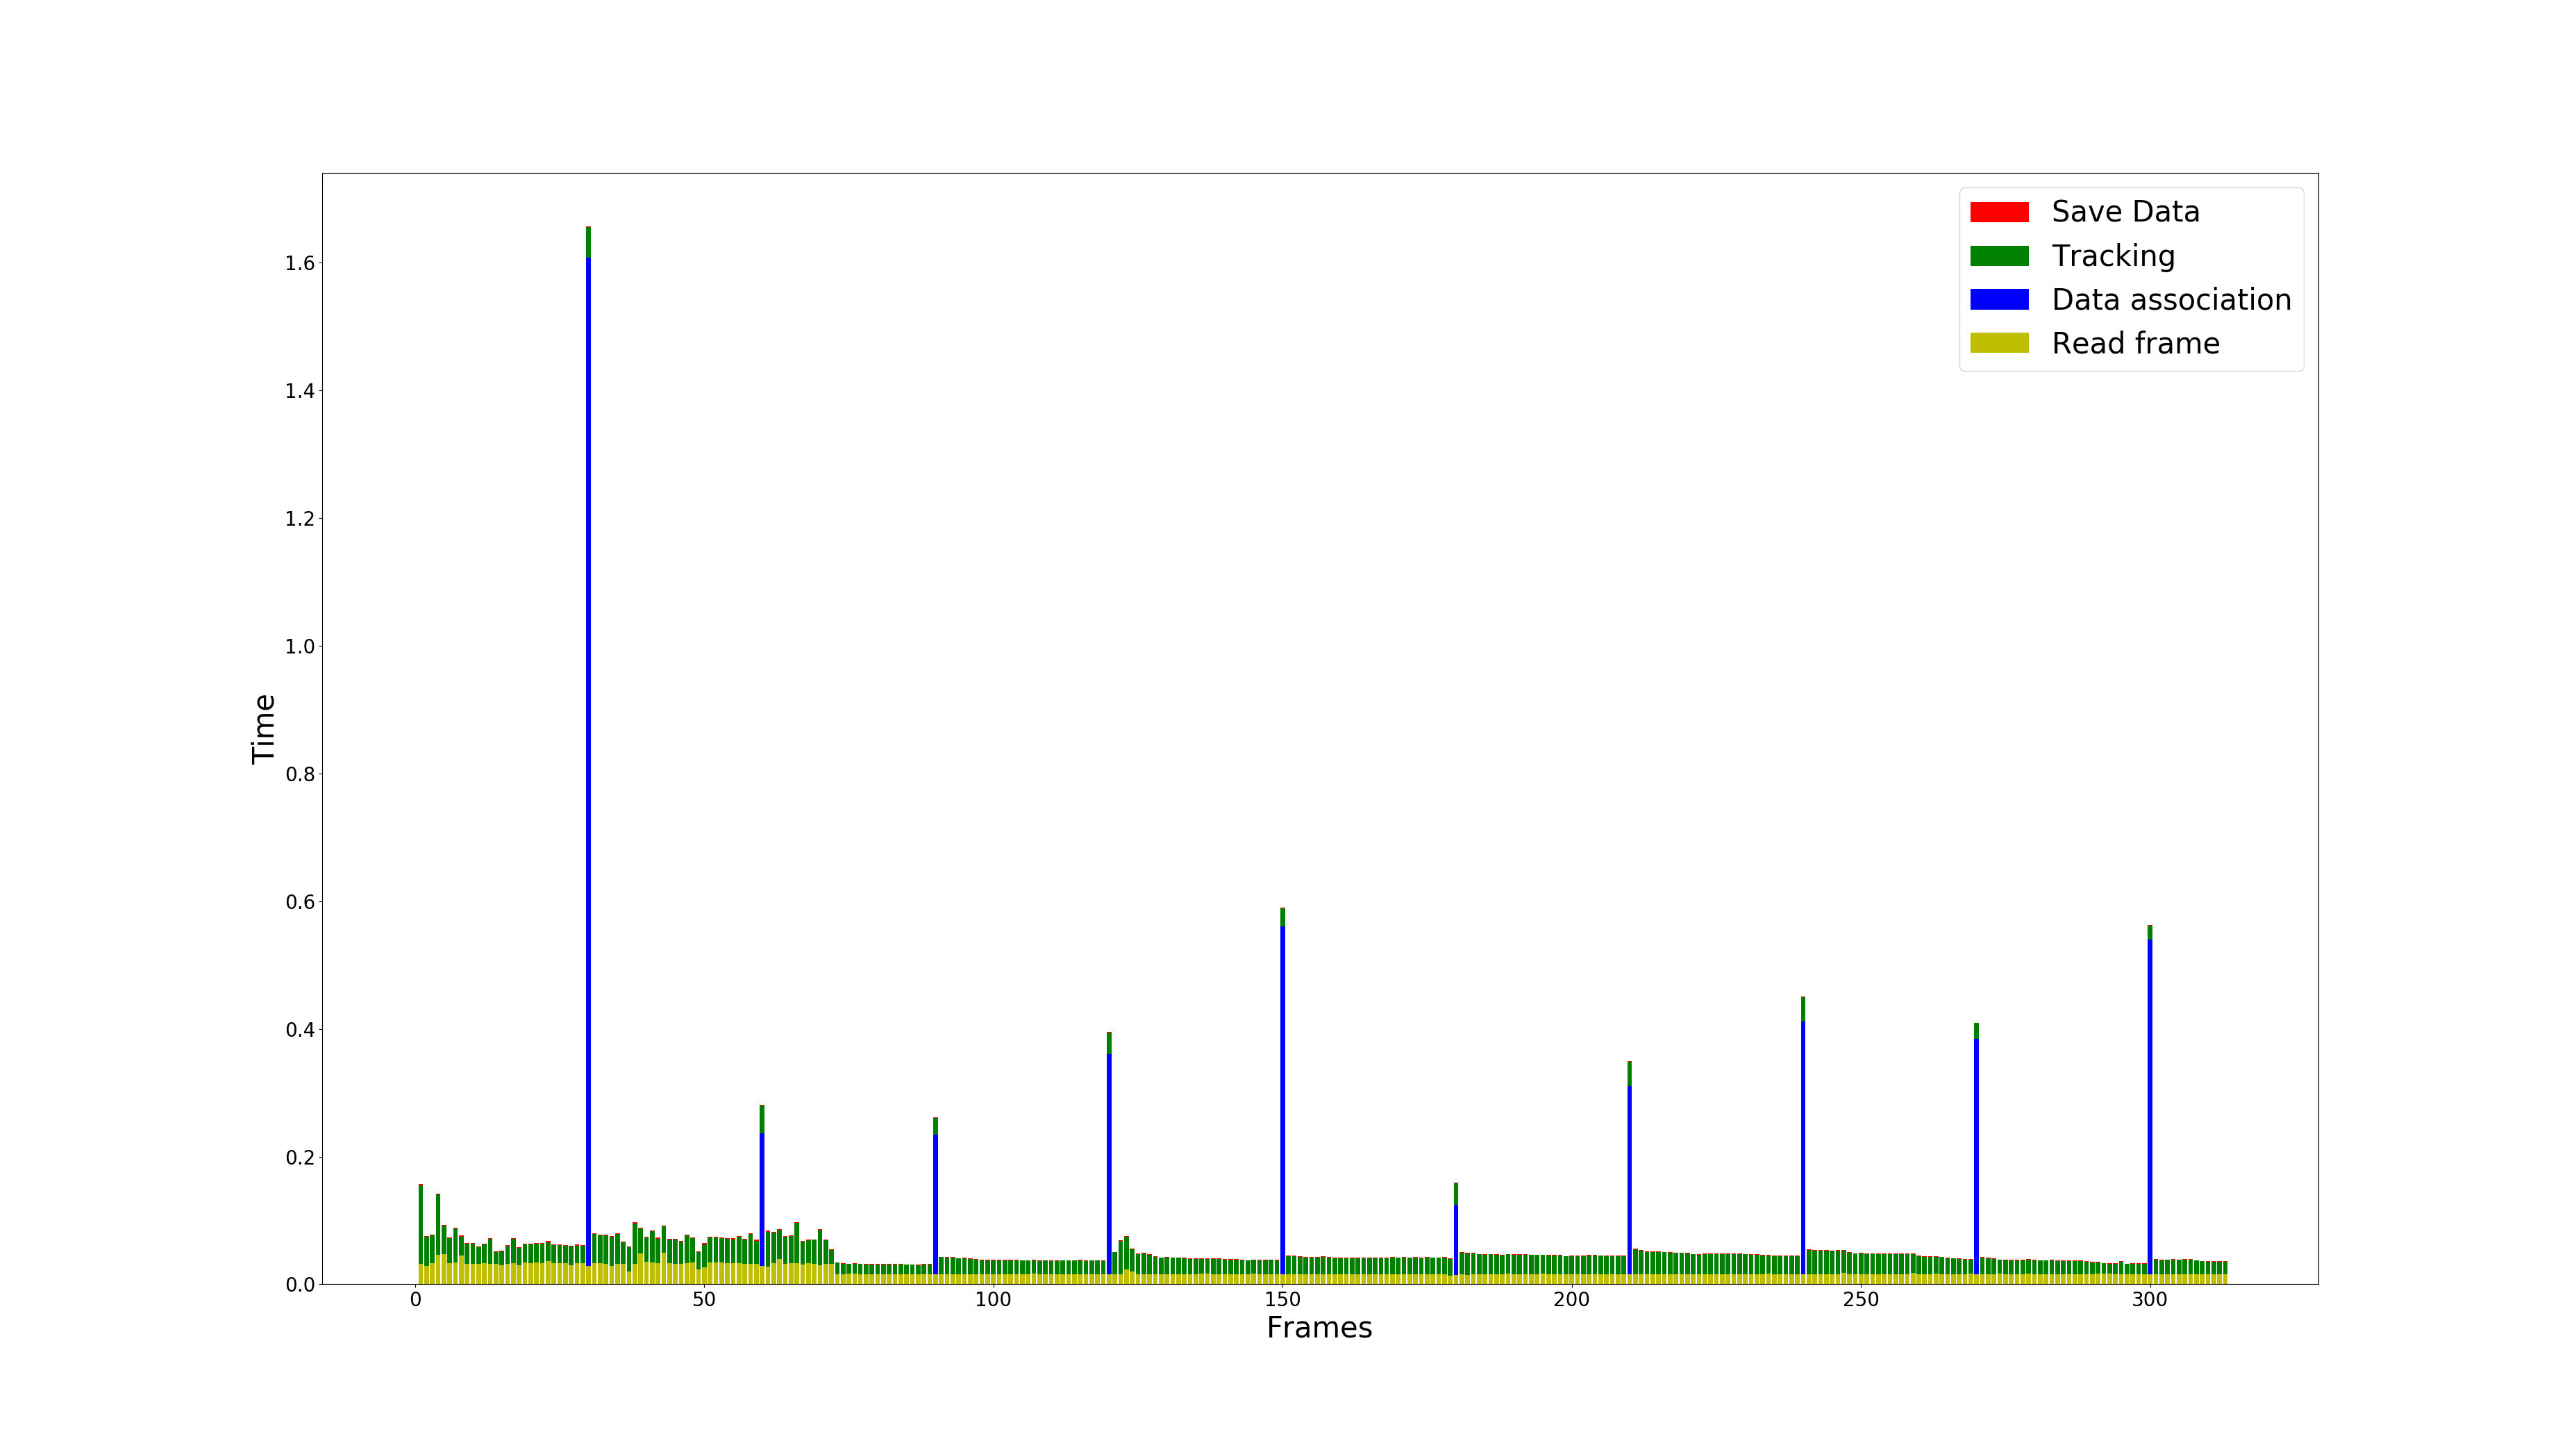
\includegraphics[width=0.9\linewidth]{graphicsRearrange/temps/timeGenral.png}
\caption{Barplot of the timming.} \label{timing1}
\end{figure}

Getting a zoom in of the graph \ref{timing2}, we can observe when the object detector execution finishes around the frame $75$, then the execution time of the algorithm decresases, the time of reading the frame remain constant, and the tracking gets a peak after the detection and afterwards decreases this is due it erase trackets with the lost mechanism. 

\begin{figure}[H]
\centering         
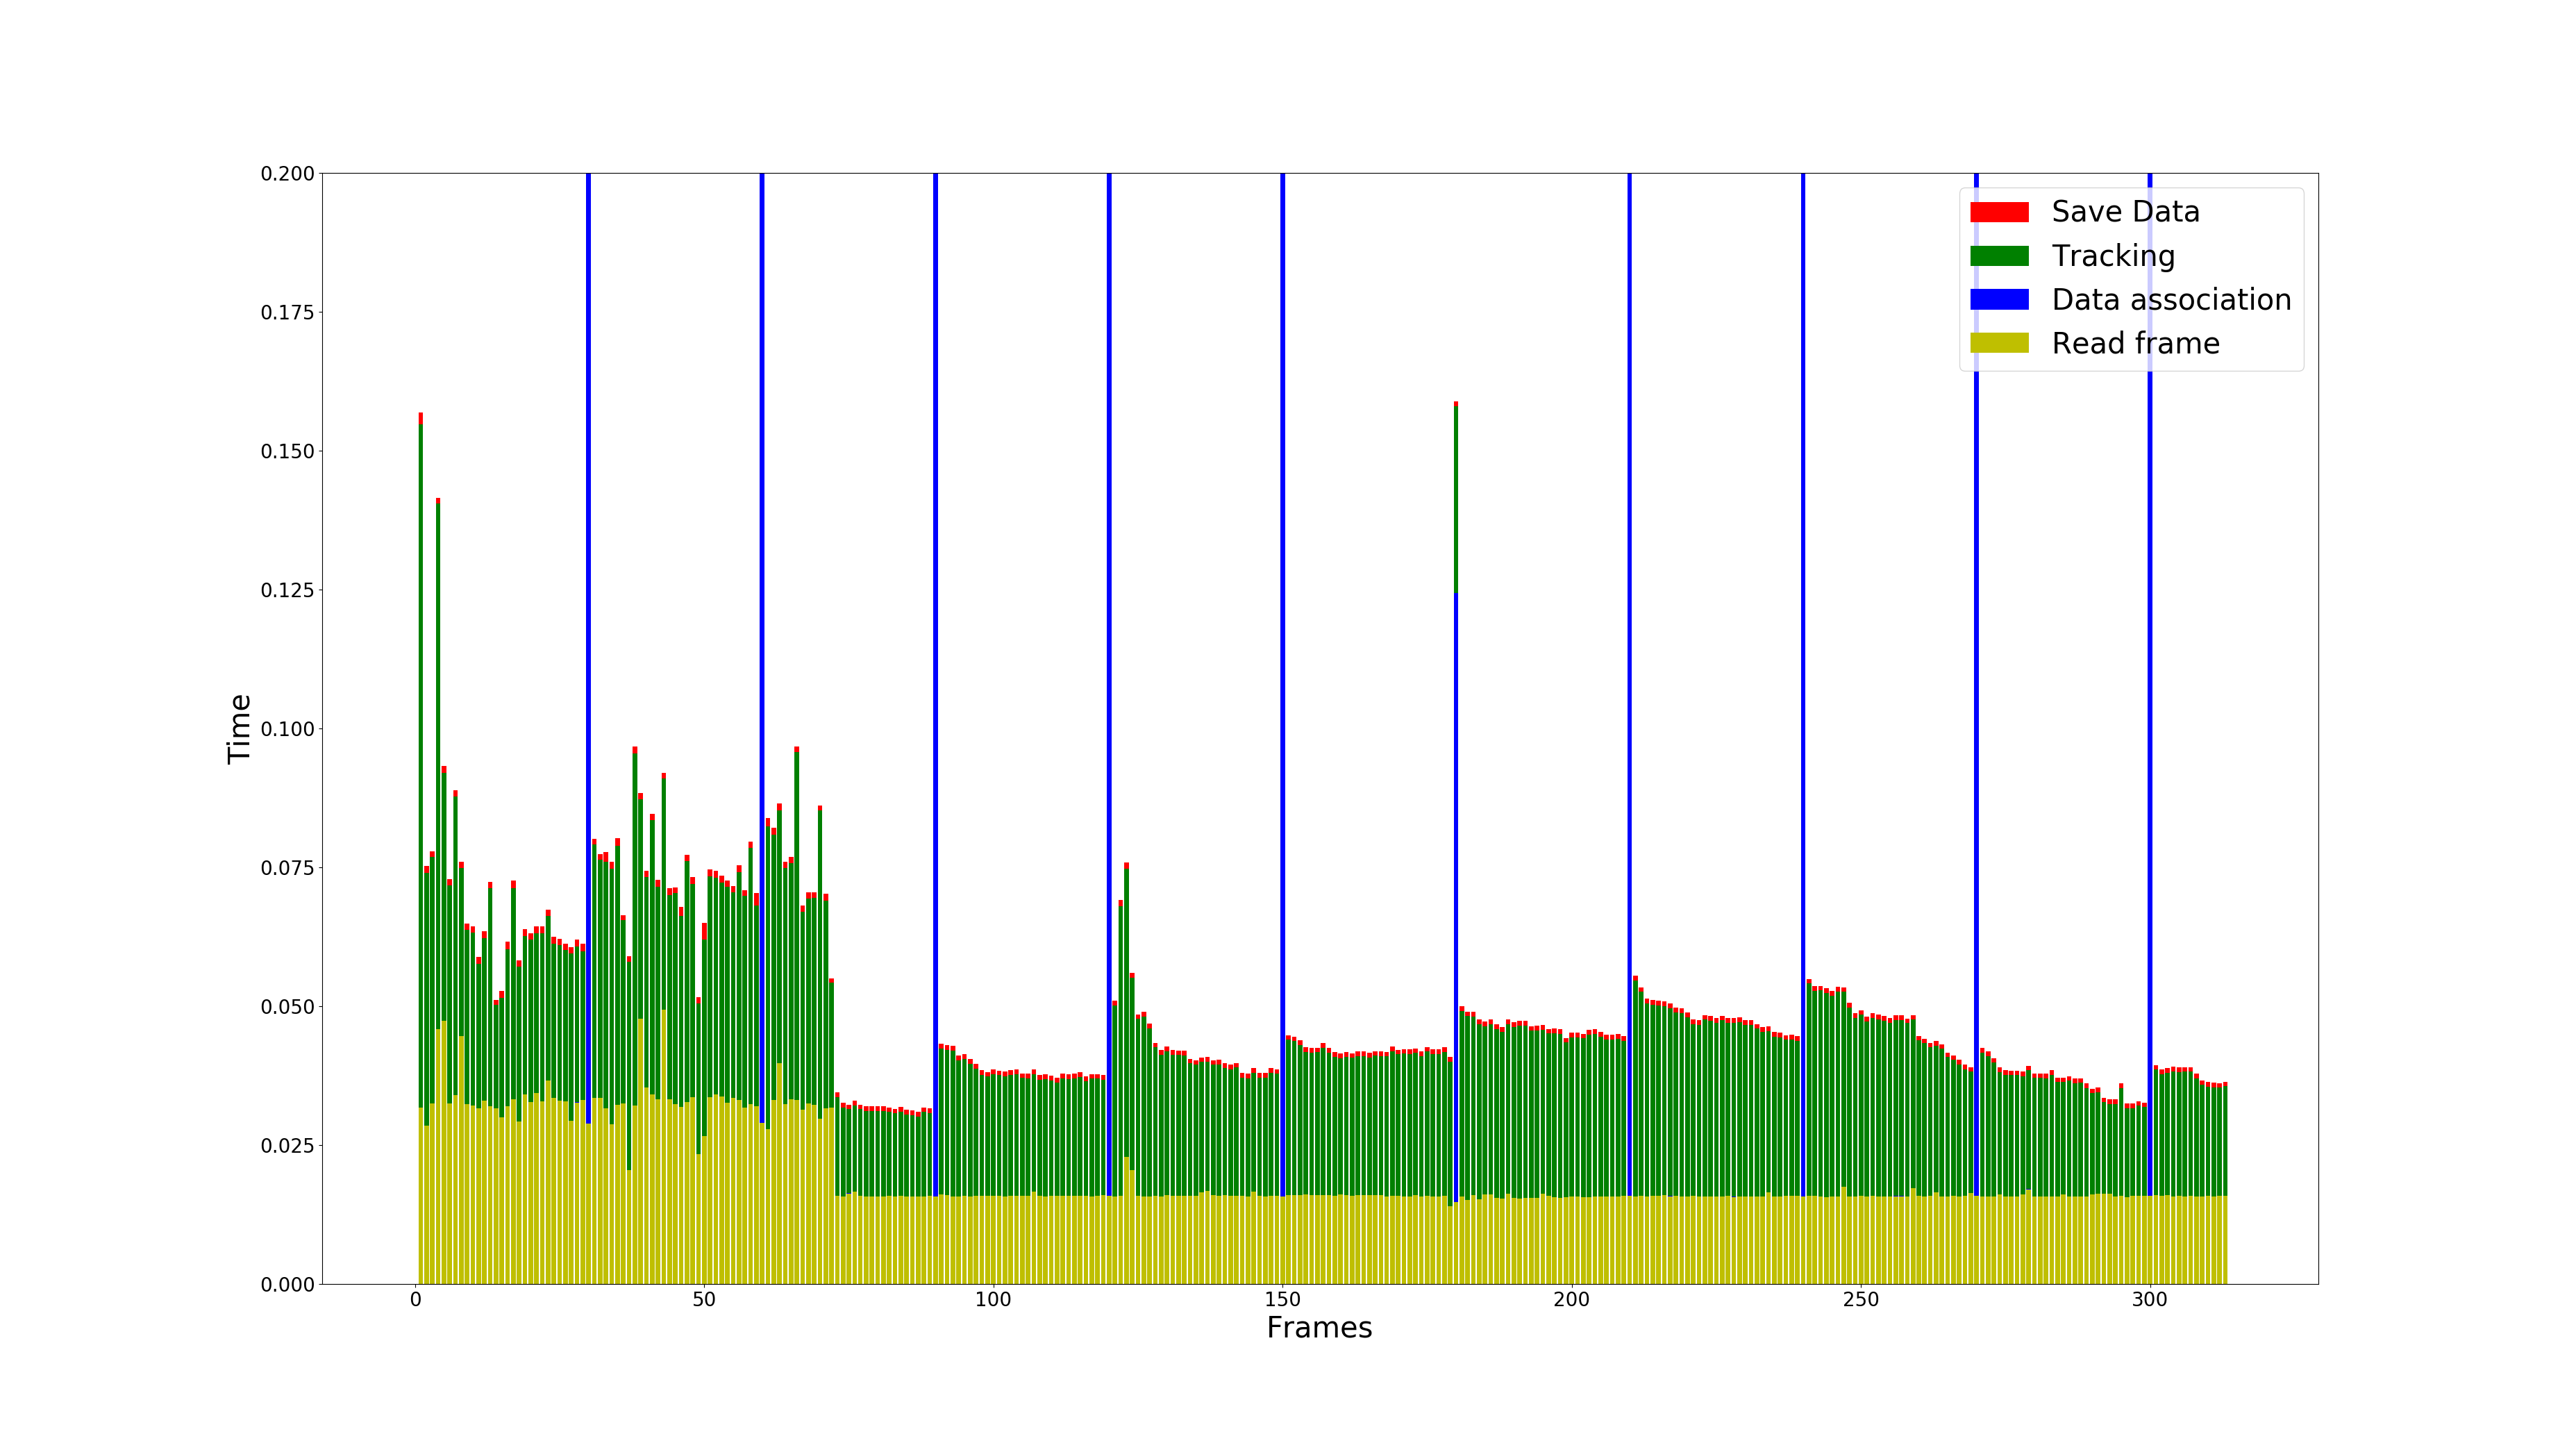
\includegraphics[width=0.9\linewidth]{graphicsRearrange/temps/timeSpecfici.png}
\caption{Zoom in of the barplot.} \label{timing2}
\end{figure}

To optimize our code we studied how to reduce the execution time of the tracking module, plotting the execution time against some dependent variables, in this case, the number of points and the size of the ROI, as we can observe in figure \ref{timing2}. We notice that the execution time is high correlated with the size of the pedestrian's ROI and not with the number of points. The main responsable is the OpenCV's routine \texttt{calcOpticalFlowPyrLK()}, but we could not modify this parameter, and reducing the number of points would have a remarkable importance in the execution time. 



\begin{figure}[H]
		
\centering

\subfigure[Points vs time.]{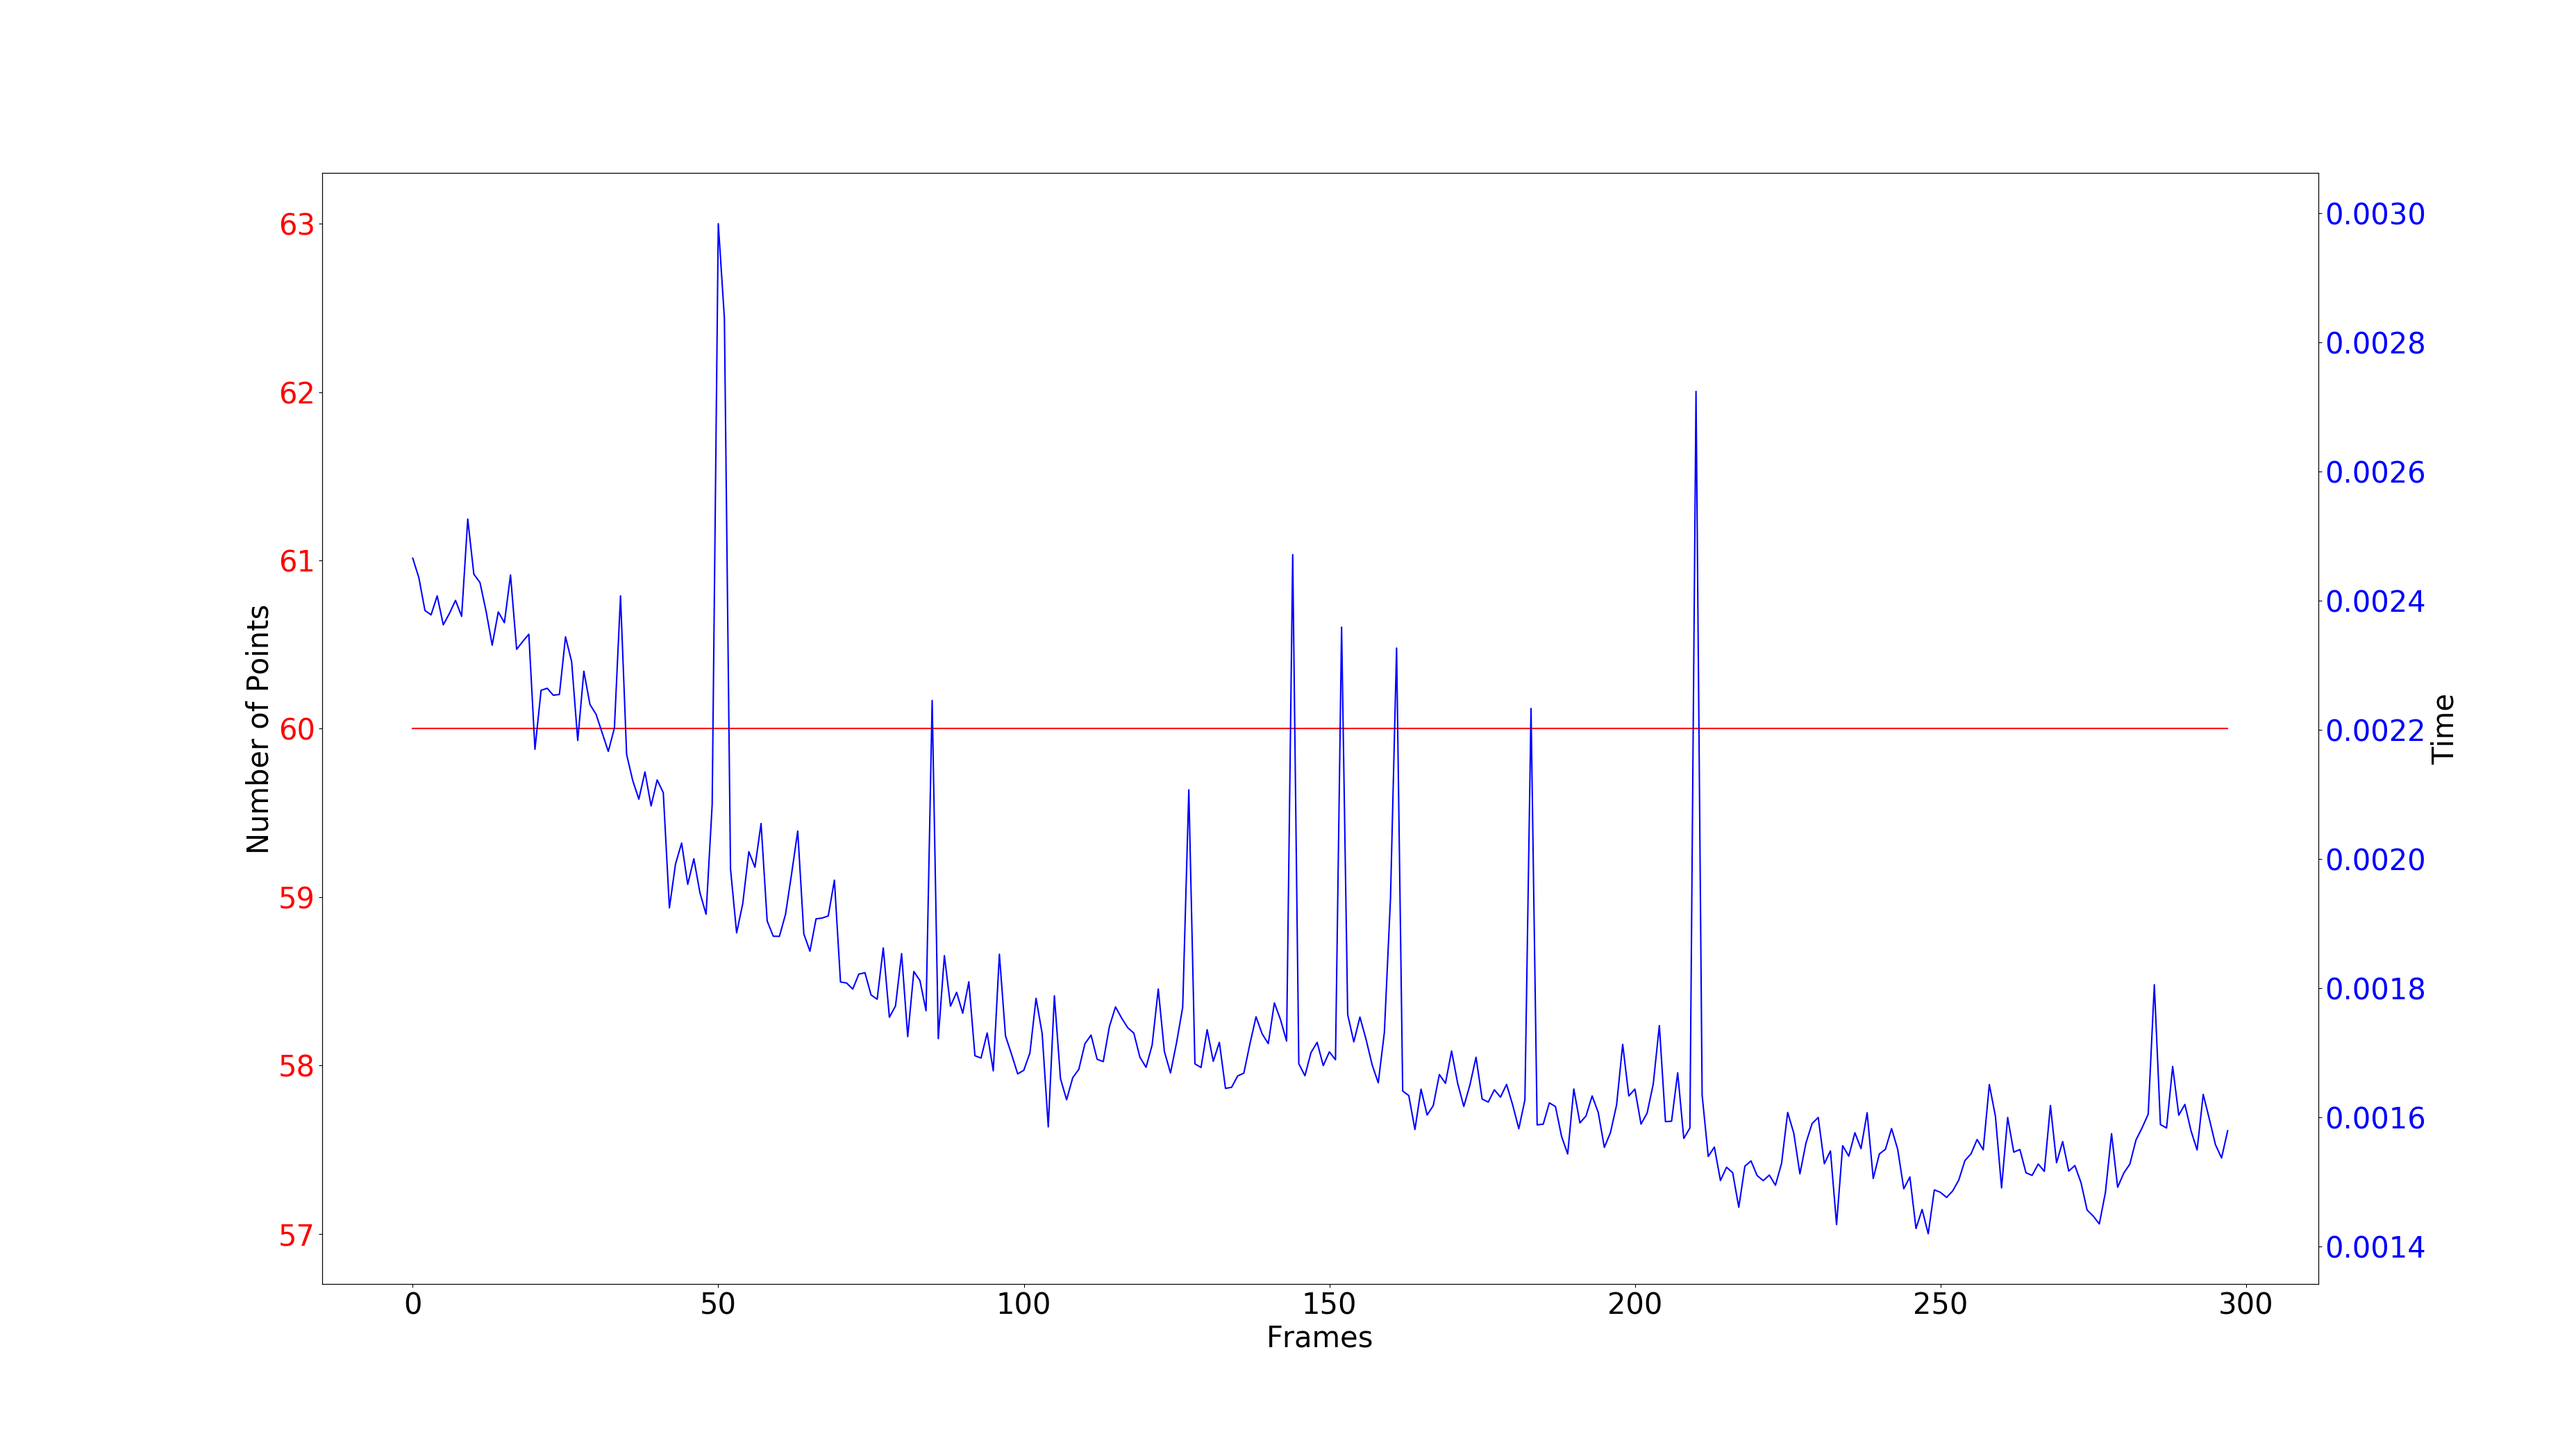
\includegraphics[width=7.2cm]{graphicsRearrange/points/points1.png}}
\subfigure[Size ROI vs time.]{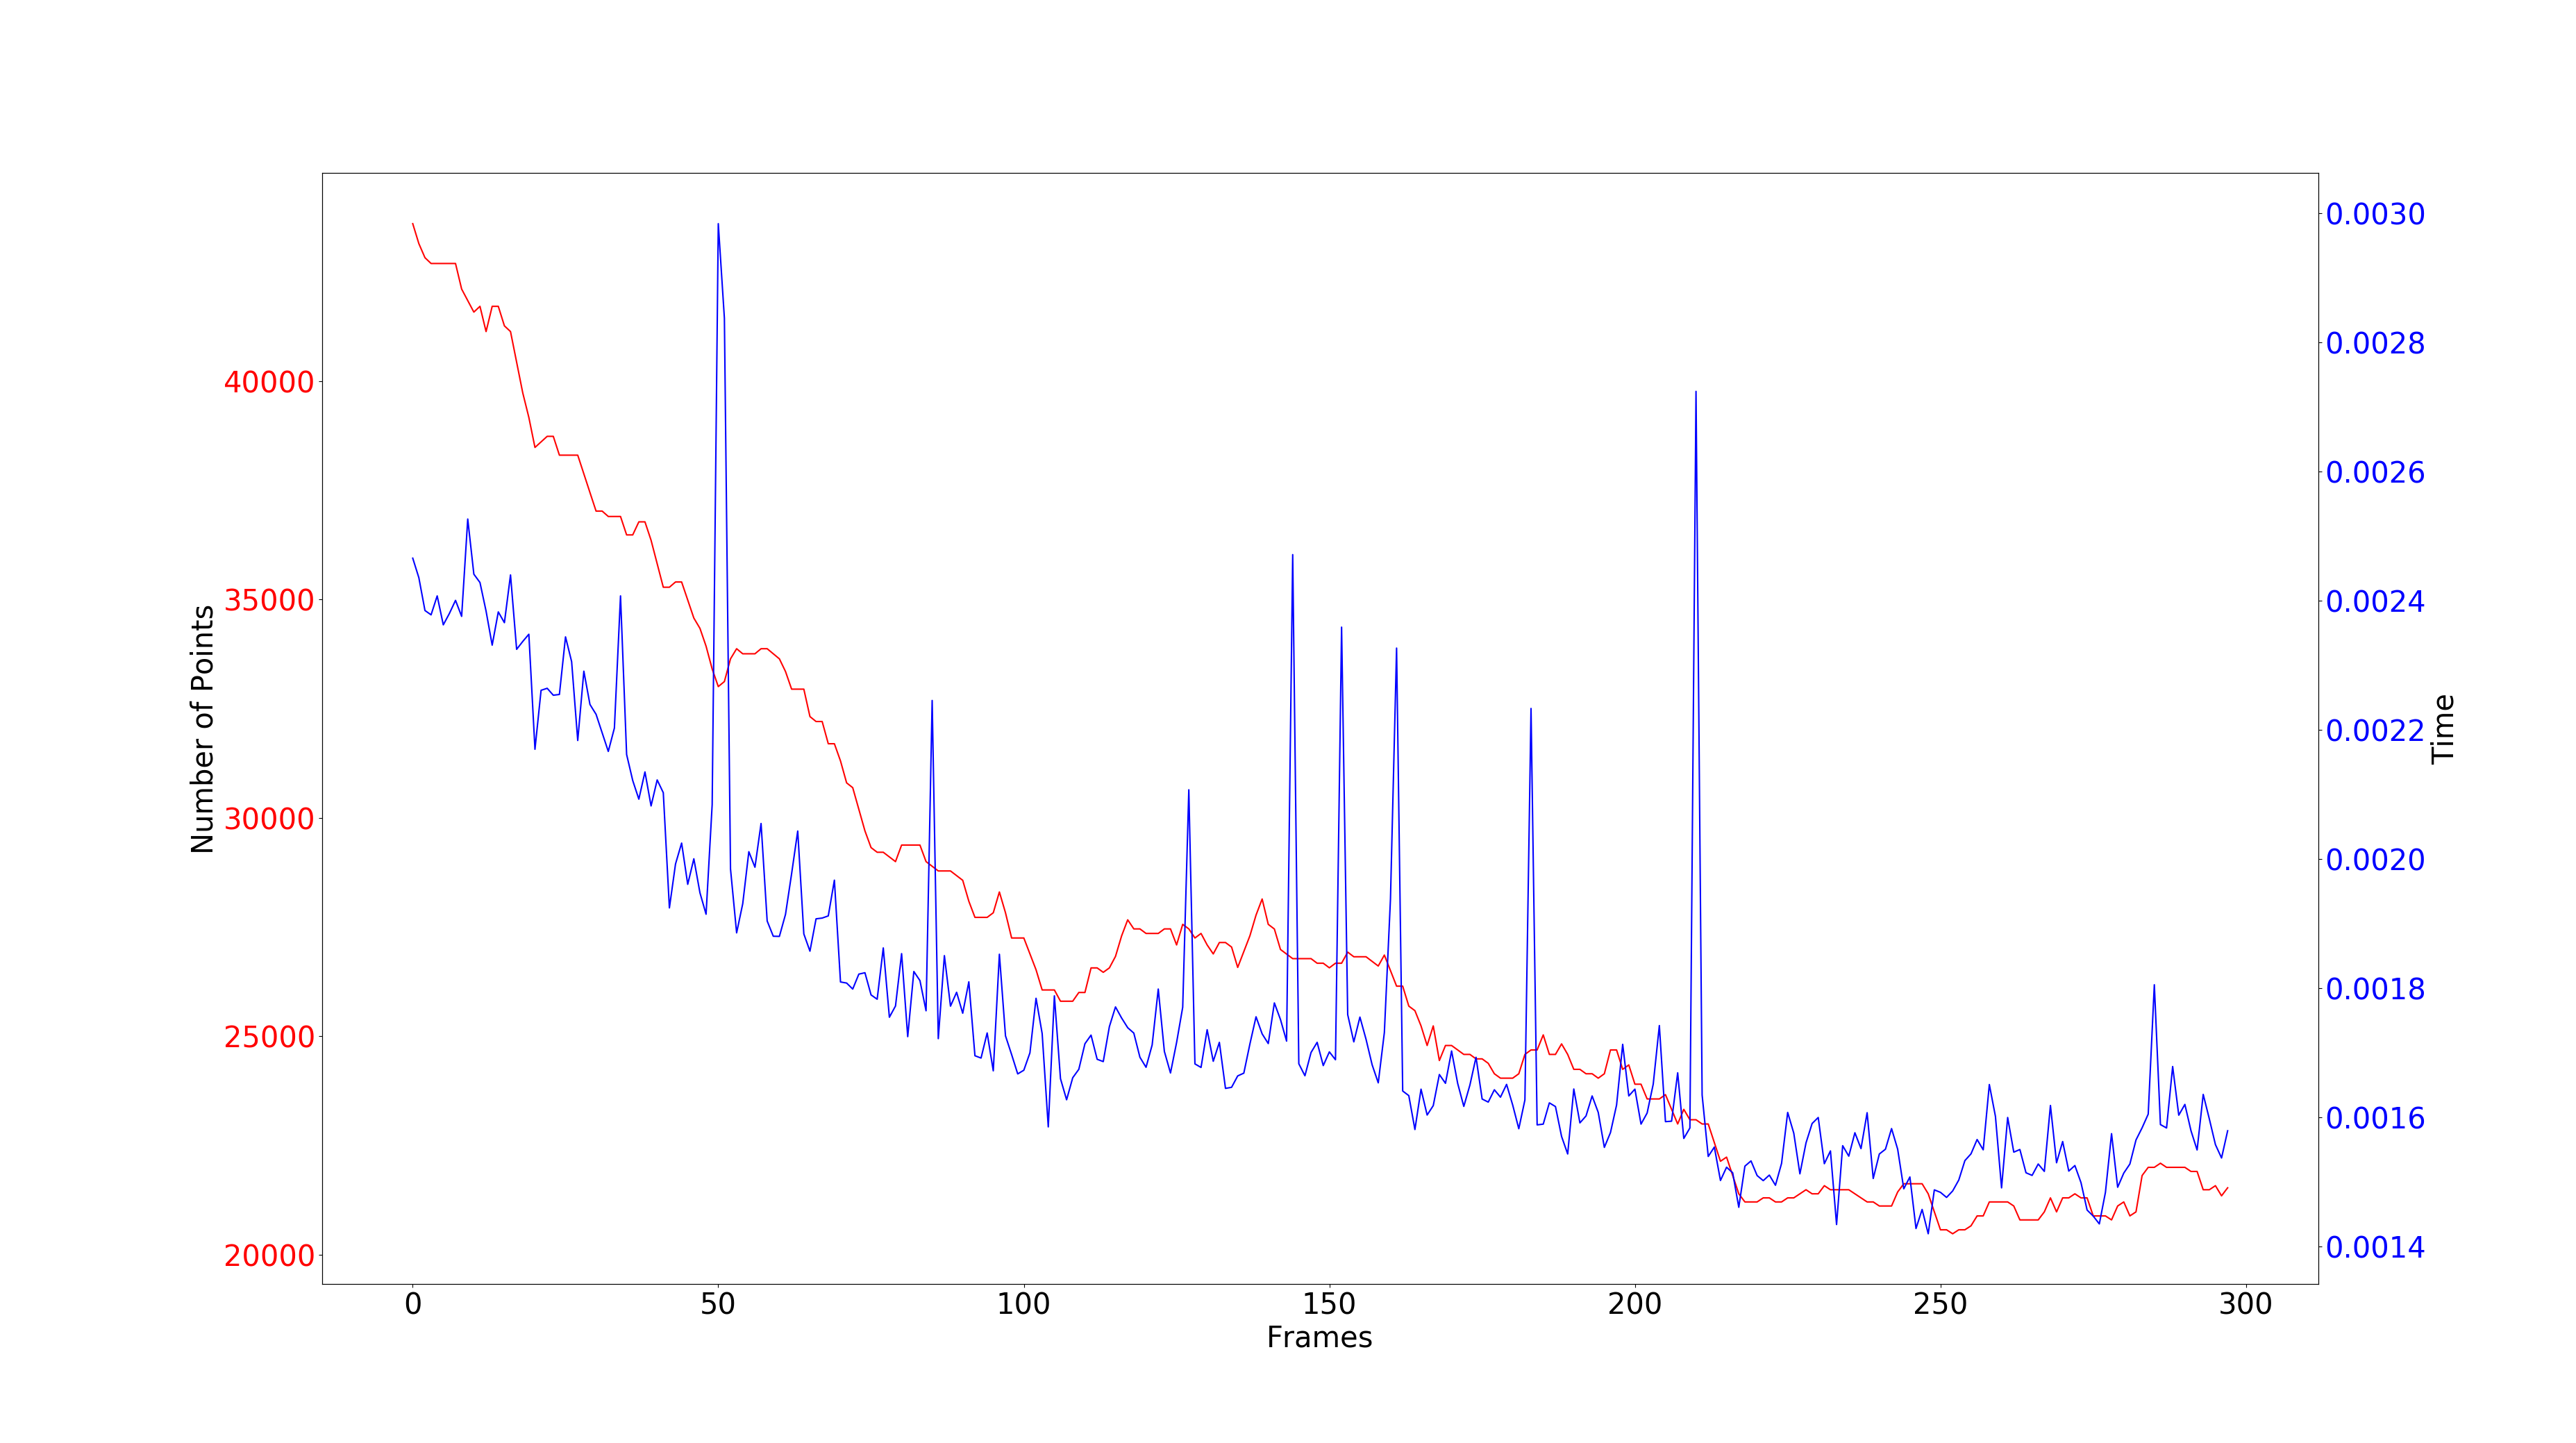
\includegraphics[width=7.2cm]{graphicsRearrange/points/timss.png}}
\caption{Time versus points and size of the ROI.}
\label{timing2}
\end{figure}
